\documentclass[12pt]{article}

% TEMPLATE DEFAULT PACKAGES
\usepackage{amssymb,amsmath,amsfonts,eurosym,geometry,ulem,graphicx,caption,color,setspace,sectsty,comment,caption,natbib,pdflscape,array,adjustbox}

% ADDED PACKAGES FOR THIS MANUSCRIPT
\usepackage{palatino,newtxmath,multirow,titlesec,threeparttable,tabu,booktabs,titlesec,threeparttable,mathtools,bm,bbm,subcaption,pdflscape,tcolorbox}
% endfloat,

\usepackage{afterpage}

\usepackage[draft]{hyperref}

% FIGURES & TABLES CAPTION STYLING
\captionsetup[figure]{labelfont={bf},name={Figure},labelsep=period}
\captionsetup[table]{labelfont={bf},name={Table},labelsep=period}

% SECTION TITLE SETTINGS
\titlelabel{\thetitle.\enskip}
\titleformat*{\section}{\large\bfseries}
\titleformat*{\subsection}{\normalsize\bfseries}

% COLUMN TYPES
\newcolumntype{L}[1]{>{\raggedright\let\newline\\\arraybackslash\hspace{0pt}}m{#1}}
\newcolumntype{C}[1]{>{\centering\let\newline\\\arraybackslash\hspace{0pt}}m{#1}}
\newcolumntype{R}[1]{>{\raggedleft\let\newline\\\arraybackslash\hspace{0pt}}m{#1}}

% MARGINS AND SPACING
\normalem
\geometry{left=1.1in,right=1.1in,top=1.0in,bottom=1.0in}
\setlength{\parskip}{2.5pt}

% SPECIAL CELL 
\newcommand{\specialcell}[2][c]{%
	\begin{tabular}[#1]{@{}l@{}}#2\end{tabular}}

% NO INDENT ON FOOTNOTES
\usepackage[hang,flushmargin]{footmisc}

\begin{document}

\begin{titlepage} 
\title{{Subsidized Housing and Urban Development: Evidence from South Africa}\thanks{We are grateful to Andrew Foster, Daniel Bjorkegren, Matthew Turner, Jesse Shapiro, Brian Knight, and John Friedman for their feedback and advice.  We also thank Adelaide Steedley and the Centre for Affordable Housing and Finance in Africa as well as GeoTerraImage for generous research guidance and for providing data without which this project would not have been possible.  Any opinions and conclusions expressed herein are those of the authors and do not necessarily represent the views of the the Federal Trade Commission or its Commissioners.}}
\author{\\[3em] Benjamin Bradlow\thanks{Dept. of Sociology, Brown University, Providence, RI  E-mail: benjamin\textunderscore bradlow@brown.edu}\\
 Stefano Polloni\thanks{Dept. of Economics, Brown University, Providence, RI E-mail: stefano\textunderscore polloni@brown.edu}\\ 
  William Violette\thanks{Federal Trade Commission, Washington, DC. E-mail: william.j.violette@gmail.com} \\
 \\ 
  }
\vspace{30mm}
\date{\vspace{5mm}This Version: \today}
\maketitle
\begin{abstract}

	Does subsidized housing improve neighborhood quality in developing countries? We estimate economic spillovers from a large public housing program in South Africa using geocoded deeds records, housing density, and census data.  To identify project impacts, we compare constructed and unconstructed projects at fine geographic levels using a difference-in-differences design.  Within project footprints, housing quality improves and subsidized formal structures successfully crowd-out slums. Yet just outside of project footprints, we detect no change in housing quantity, quality, or price. 

 %\\
%\vspace{0in}\\
%\textbf{Keywords:} traffic externalities; street livability; urban policy; housing market.\\
%\vspace{0in}\\
%\textbf{JEL Codes:} O18; H4; R2; R4.\\
\bigskip
\end{abstract}
\setcounter{page}{0}
\thispagestyle{empty}
\end{titlepage}
\pagebreak \newpage

\spacing{1.4}
\section{Introduction} \label{sec:introduction}

In developing countries, 30\% of urban populations live in crowded slums where households often suffer from unsanitary conditions and high crime rates \citep{mdg}. Combined with low infrastructure access and insecure property rights, these negative congestion externalities are thought to pose long-lasting obstacles to upward mobility and local economic development \citep{10.1257/jep.27.4.187}. We study a common policy response where governments replace slums with serviced formal structures and move slum dwellers into public housing projects. These programs aim to provide not only direct health and economic benefits to recipients, but also greater incentives for neighbors to invest in their homes and communities, reducing negative externalities and steering residents away from poverty traps. At the same time, subsidized housing can attract slums by improving nearby access to bulk services like water and sanitation, as well as providing under-utilized developpable land within project areas. These indirect housing opportunies are especially salient in South Africa, where {\it backyarding} is a common and widely documented form of land use.\footnote{see recent work by \cite{Brueckner2018backyarding}} In this way, public housing programs may ultimately exacerbate the same negative externalities they were designed to remediate. While much of the existing literature has focused on estimating direct recipient impacts \citep{cattaneo2009housing,franklin2016enabled,galiani2017shelter}, the broader consequences of subsidized housing for urban development remain poorly understood.

% While these policies aim to reduce slum growth
%While these policies are often motivated by immediate health and economic benefits for recipients, economic theory emphasizes how public housing can provide incentives for neighbors to invest more in their own homes and communities, reducing negative externalities and steering communities away from poverty traps.{}
% In this paper, we document another
% We find that these policies can have 

%In this paper, we analyze the impacts of public housing on the development of surrounding neighborhoods.

In this paper, we estimate economic spillovers from a large-scale housing program in South Africa, focusing on the quality, density and price of nearby housing. With over 3 million allocated dwellings, the program is one of the largest in the developing world, and continues to respond to large backlogs in demand \citep{dhsreports}. The program aims not only to serve as ``a key strategy for poverty alleviation'' to direct beneficiaries, but also to generate community-wide benefits, ``leveraging growth in the economy, [...] combating crime, promoting social cohesion, [...] and utilizing housing as an instrument for the development of sustainable human settlements, in support of spatial restructuring'' \citep{bng}. 

We combine administrative records for 57completed housing projects in the province of Gauteng, with data on property transactions, formal and informal housing densities, and dwelling characteristics to measure the local impact of these projects.   We find evidence of greater access to services, improved home quality, and a greater share of formal housing stock within project areas but no effects on surrounding areas.  Examining nearby housing transactions, we find no statistically significant effects of public housing on prices in the formal market.  To interpret these findings, we provide a simple conceptual framework balancing the amenity effects of improved housing quality against the price and quantity effects of a housing supply shock.  This framework helps shed light on the absence of spillover effects detected in our analysis.

% the welfare effects..
% attribute the local decline in housing prices in the formal market to greater externalities imposed 
% To understand the welfare implications of this policy, we also develop a model similar to... 
%We then use heterogeneity in the extent to which projects eradicate existing slums as a natural experiment to quantify negative externalities from slum areas.  Our estimates imply that increasing slum density by [XX]\% leads to a [XX]\% decline in local housing prices.  We find some evidence that this effect scales non-linearly with the size of the housing projects, which has theoretical implications for the extent to which slum areas represent poverty traps.

Our empirical estimates rely on a difference-in-differences design leveraging both the timing of housing project construction as well as the precise geography of treated areas. Like prior studies in the US, the substantial uncertainty in project timing due to difficulties coordinating many stakeholders and sources of funding limits the extent to which local housing markets are able to anticipate the projects \citep{diamond2016wants, serihistory}.  To address the potential endogenous placement of housing projects, we use 60planned but unconstructed projects as counterfactuals and detect no impacts of these projects on local housing markets.

\begin{comment}
Our zero spillover estimates stand in contrast to a large literature in development that has found positive impacts of public housing on direct recipients.  Relying on small-scale experimental designs, previous studies have linked public housing to improvements in employment outcomes \citep{franklin2016enabled}, self-reported wellbeing \citep{galiani2017shelter, devoto2012happiness}, and child health outcomes \citep{cattaneo2009housing}.  Data limitations both in finding a large enough sample of housing projects and in identifying outcomes at a precise spatial scale have prevented previous studies from identifying spillover effects.  Taken alongside these previous studies, our findings suggest that policymakers may be able to continue emphasizing direct benefits to recipients in designing future housing policy since spillover affects appear to be minimal.
\end{comment}

We proceed by first providing background on the South African housing program in Section~\ref{section:background}.  In Section~\ref{section:model}, we develop a conceptual framework of housing supply and housing externalities to help interpret the results. Section~\ref{section:data} describes the data used to measure outcomes and details our approach to identifying housing projects while Section~\ref{section:descriptives} provides descriptive evidence.  We present spillover results for residential home prices in Section~\ref{section:resultsprices} and demographic outcomes in Section~\ref{section:resultscensus}.  Section~\ref{section:discussion} includes a discussion of our findings before providing some concluding thoughts.


\section{Subsidized Housing in South Africa} \label{section:background}

The projects studied in this paper were implemented as part of a large national housing subsidy scheme enacted in 1994. Though periodically revised and renamed,\footnote{Public housing in South Africa has been delivered under the {\it Reconstruction and Development Program} (RDP) starting in 1994 and subsequently by its successor, {\it Breaking New Grounds}, as of 2004.} the program has consistently sought to redress the economic and geographic legacy of apartheid by providing formal housing to low-income households. Subsidized housing efforts at the national level have focused on constructing and allocating 40m$^2$, single-story, two-room dwellings in groups of 50 to 500 per project. According to government figures, upwards of 3 million housing units have been delivered between 1994 and 2015.

\subsection{Planning and Delivery}

Housing projects are primarily located on undeveloped state-owned land although in some cases, municipalities work with private developers to purchase inexpensive, vacant private land for these projects.  Finding suitable land plots often requires policymakers to locate these projects far from city centers and economic opportunities \citep{dhsreports}.  Undeveloped land plots may contain preexisting informal settlements, which the government tries to replace with new formal houses and ensure that preexisting residents benefit from the new project houses \citep{serihistory}.

Facing substantial housing demand, the Department of Human Settlements has continued to issue grants to provincial governments to maintain yearly housing allocations \citep{dhsreports}.  While the location and types of projects are determined by provincial and municipal governments, construction is subcontracted to private developers who also act as project managers assisting in the allocation of houses to beneficiaries \citep{seriq}.

Since housing projects require coordination between many stakeholders, these projects often face unanticipated delays and cancellations due to labor and land procurement issues, difficulties gaining support from local government agencies, environmental impact assessments, and inadequate bulk infrastructure provision \citep{dhsreports}.  In one example, political disagreements with local stakeholders led to the abandonment of a large project near Johannesburg \citep{protest}.  In other cases, housing projects have been delayed for upwards of 10 years \citep{dagpl}. 


\subsection{Recipients}

The National Department of Human Settlements issues guidelines for eligibility and maintains an official waiting list for eligible households.  Eligibility requires citizenship, no previous property ownership, being married or having financial dependents, and having a monthly household income below R3,500 \citep{seriq}.\footnote{The Gauteng Province has implemented their own waiting list since 2008 in order to exert greater control over the allocation process.}  The share of households reporting at least one member on the waiting list has remained stable at over 13\% from 2009 to 2013.\footnote{\label{GHSnote}This figure is calculated from the General Household Surveys from 2009 to 2013}  Before construction, each project is assigned beneficiaries in a first-come, first-served basis according to the waiting list in their province or municipality.  For in-situ upgrading projects, previous inhabitants of informal settlements receive renovated houses while any remaining houses are allocated according to the housing waiting list.

In practice, these guidelines are loosely followed.  Recent reports point to cases of corruption in the allocation of houses while in some instances, housing projects are organized with the assistance of local community groups who ultimately select the beneficiaries \citep{seriq}; \citep{casestudytinazonke}.  Research suggests that beneficiaries are often selected over the course of project construction and sometimes even after construction has finished \citep{seriq}. Beneficiaries are expected to pay a small one-time payment in order to receive title for their houses.  Guidelines also prevent beneficiaries from reselling their houses within their first 7 years of ownership.  Despite these guidelines, only 82\% of project houses are reported being still occupied by their original beneficiaries within five years of construction.\textsuperscript{\ref{GHSnote}} Anecdotal evidence suggests that project managers are aware of active secondary markets but have difficulty policing these transactions \citep{resale}.

\subsection{Backyard Shacks}

By design, subsidized housing in South Africa offers recipients generous amounts of yard space, which often serve alternative land uses. The construction of informal backyard shacks is a common occurrence within project boundaries. Recipients typically enter agreements with tenants (at times relatives) to lease the shacks for cash or in-kind payments. According to the 2011 census, backyard tenants represent 7.5\% of South African households.\footnote{This figure jumps to 12.5\% for the province of Gauteng, where our study is conducted.} Though the structures are not as durable as their government-provisioned counterparts, living conditions are typically superior than those of conventional informal settlements. Tenants gain indirect access to their landlord's services such as water taps, electricity connections, and toilets, and benefit from reduced eviction threats and greater personal safety \citep{beall2003social}. \cite{Brueckner2018backyarding} note that {\it backyarding} is suggestive of inefficiencies in the program delivery, and allows to correct potential misallocations of resources. Importantly for our analysis, backyard shacks reveal that more household benefit from subsidized housing than the number of direct recipients. According to the general household surveys (2009-2013), more than 33\% of government-provisioned homes have backyard shacks within two years of the delivery date. 

\section{Conceptual Framework}\label{section:model}

Stay tuned.

\begin{comment}
We consider housing projects as generating positive shocks to housing quantity as well as quality.  Following a standard model of housing supply and demand, increases in formal housing quantity should (1) lower prices of formal housing nearby and (2) incentivize households to move into project areas, both leading to increases in population.  At the same time, gains in housing quality not only benefit direct recipients, but also may have an amenity effect, increasing the desirability of living in neighboring areas \citep{diamond2016wants}.  This amenity effect is likely to (1) increase house prices nearby and (2) drive increases in local population as well.  Taken together, quantity and quality effects have ambiguous predictions for formal housing prices nearby but both predict increases in population both within and around housing project areas.

This simple framework ignores additional features specific to housing markets in developing countries.  In the housing production function, there may be complementarities or substitution between project housing and informal housing.  By zoning and servicing large swaths of land, housing projects may lower the cost of building new informal housing settlements both within and around these projects.  At the same time, clearly defined property rights allocated by these housing projects may increase the cost of squatting, decreasing nearby informal settlements.

The level of informal settlement growth generated by these housing projects may have additional welfare consequences due to general externalities from slum growth \citep{10.1257/jep.27.4.187}.  Health effects, congested infrastructure, and higher crime combine to form negative amenities, potentially depressing nearby housing prices or lowering population densities in these areas.  Although these specific mechanisms are difficult to precisely identify in this setting, these considerations motivate analyzing the differential impacts of housing projects for informal versus formal housing.
\end{comment}

\section{Data Sources}\label{section:data}

Our analysis focuses on the South African province of Gauteng, both the smallest geographically and most populated province in the country. Gauteng's boundaries roughly correspond to the greater metropolitan area of Johannesburg and Pretoria. Understanding the local development impacts of public housing requires (1) outcomes measured at high spatial resolutions, and (2) a precise measure of the location, timing, and size of housing projects.  To this end, we rely on four main data sources: administrative maps describing Gauteng's housing policies, deeds data on housing transactions, household-level census data, and building-based land use information. Each is described in turn below.

\subsection{Deeds Data and Location of Housing Projects}

 We locate housing projects using a combination of administrative policy maps and deeds data. We obtain the former from the Gauteng City Regional Observatory, a research unit joint with the Gauteng Provincial Government and two Johanesburg universities.\footnote{\href{url}{www.gcro.ac.za/}} The maps describe 642planned housing projects as of 2008, including (on some occasions) notes on their completion status.\footnote{Since this data comes in the form of overlapping shapefiles, we use the union of intersecting shapes, excluding small shapes below 0.5 km$^2$.} The latter is sourced from the South African National Deeds Office, covering the 2001 to 2011 universe of transactions in {\it affordable areas}, defined as census enumeration areas with 2010 mean house prices below R500,000. These data were kindly provided by the Affordable Land and Housing Data Centre, which tracks affordable housing markets. Transaction information includes sale price, GPS location, plot size, buyer name, and seller name.


\begin{table}[h!]
\vspace{4mm}
\caption{Top-Five Sellers in Housing Transactions Sample}\label{table:topfivesellers}
\vspace{-2mm}
\centering
\begin{tabu}{lc}
\toprule
 Seller Name & Observations \\
\midrule
City Of Johannesburg Metropolitan Municipality & 29,087  \\
City Of Johannesburg & 27,672  \\
City Of Tshwane Metropolitan Municipality & 24,780  \\
Ekurhuleni Metropolitan Municipality & 21,758  \\
Gauteng Provincial Housing Advisory Board & 13,058  \\
{\bf Total Observations }& {\bf 549,704}  \\
\bottomrule
\end{tabu}

\vspace{-4mm}
\end{table}

 \subsubsection*{Constructed Housing Projects}

 Using the administrative policy maps, we define projects as successfully constructed when we observe recipients receiving deeds to their government-sponsored house within the projects boundaries. To identify state-sponsored housing transactions, we follow a filtering procedure established by our data provider. Properties are first assumed to belong to a housing project if the seller name includes a government, municipality, or large developer when first transacted. In 	\mbox{Table \ref{table:topfivesellers}}, we show that these institutional sellers represent an important share of our sample. We then exclude deeds flagged as large buildings used for commercial purposes (less than 2\% of transactions), as well as purchase prices more than R50,000 above the yearly nominal subsidy values (less than 4\% of remaining transactions). As shown in the right panel of Figure \ref{figure:transactionhist}, transaction prices for properties deemed to belong to public housing programs exhibit significant mass-points in their distribution, consistent with many properties being recorded with these subsidy values. Finally, we exclude transactions occurring in Gauteng's historic townships, because the bulk of residential construction within these areas precedes the start of South Africa's housing program.\footnote{Urban townships are apartheid-era residential areas created for black migrant workers. Township boundaries were also provided by the Gauteng City-Region Observatory.} Altogether, this filtering procedure identifies over 127,000 properties as government-sponsored housing. Overlaying theses properties' GPS coordinates with the housing policy maps, we are able to identify 57constructed housing projects. Delivery dates for the projects are then inferred from the distribution of transactions over time. Specifically, considering transactions within each projects separately, we set the modal transaction month as the delivery month for each project. Within projects, most government-sponsored properties are transacted in the same month. %This is apparent from the upper panel of figure \ref{figure:densitytime}, where monthly transaction densities for subsidized properties are plotted 36 months prior and following the modal delivery month.

\begin{figure}[t]
\caption{Transaction Price Histogram}\label{figure:transactionhist}
\centering
\tcbox[colback=white,boxrule=.35mm,boxsep=0mm]{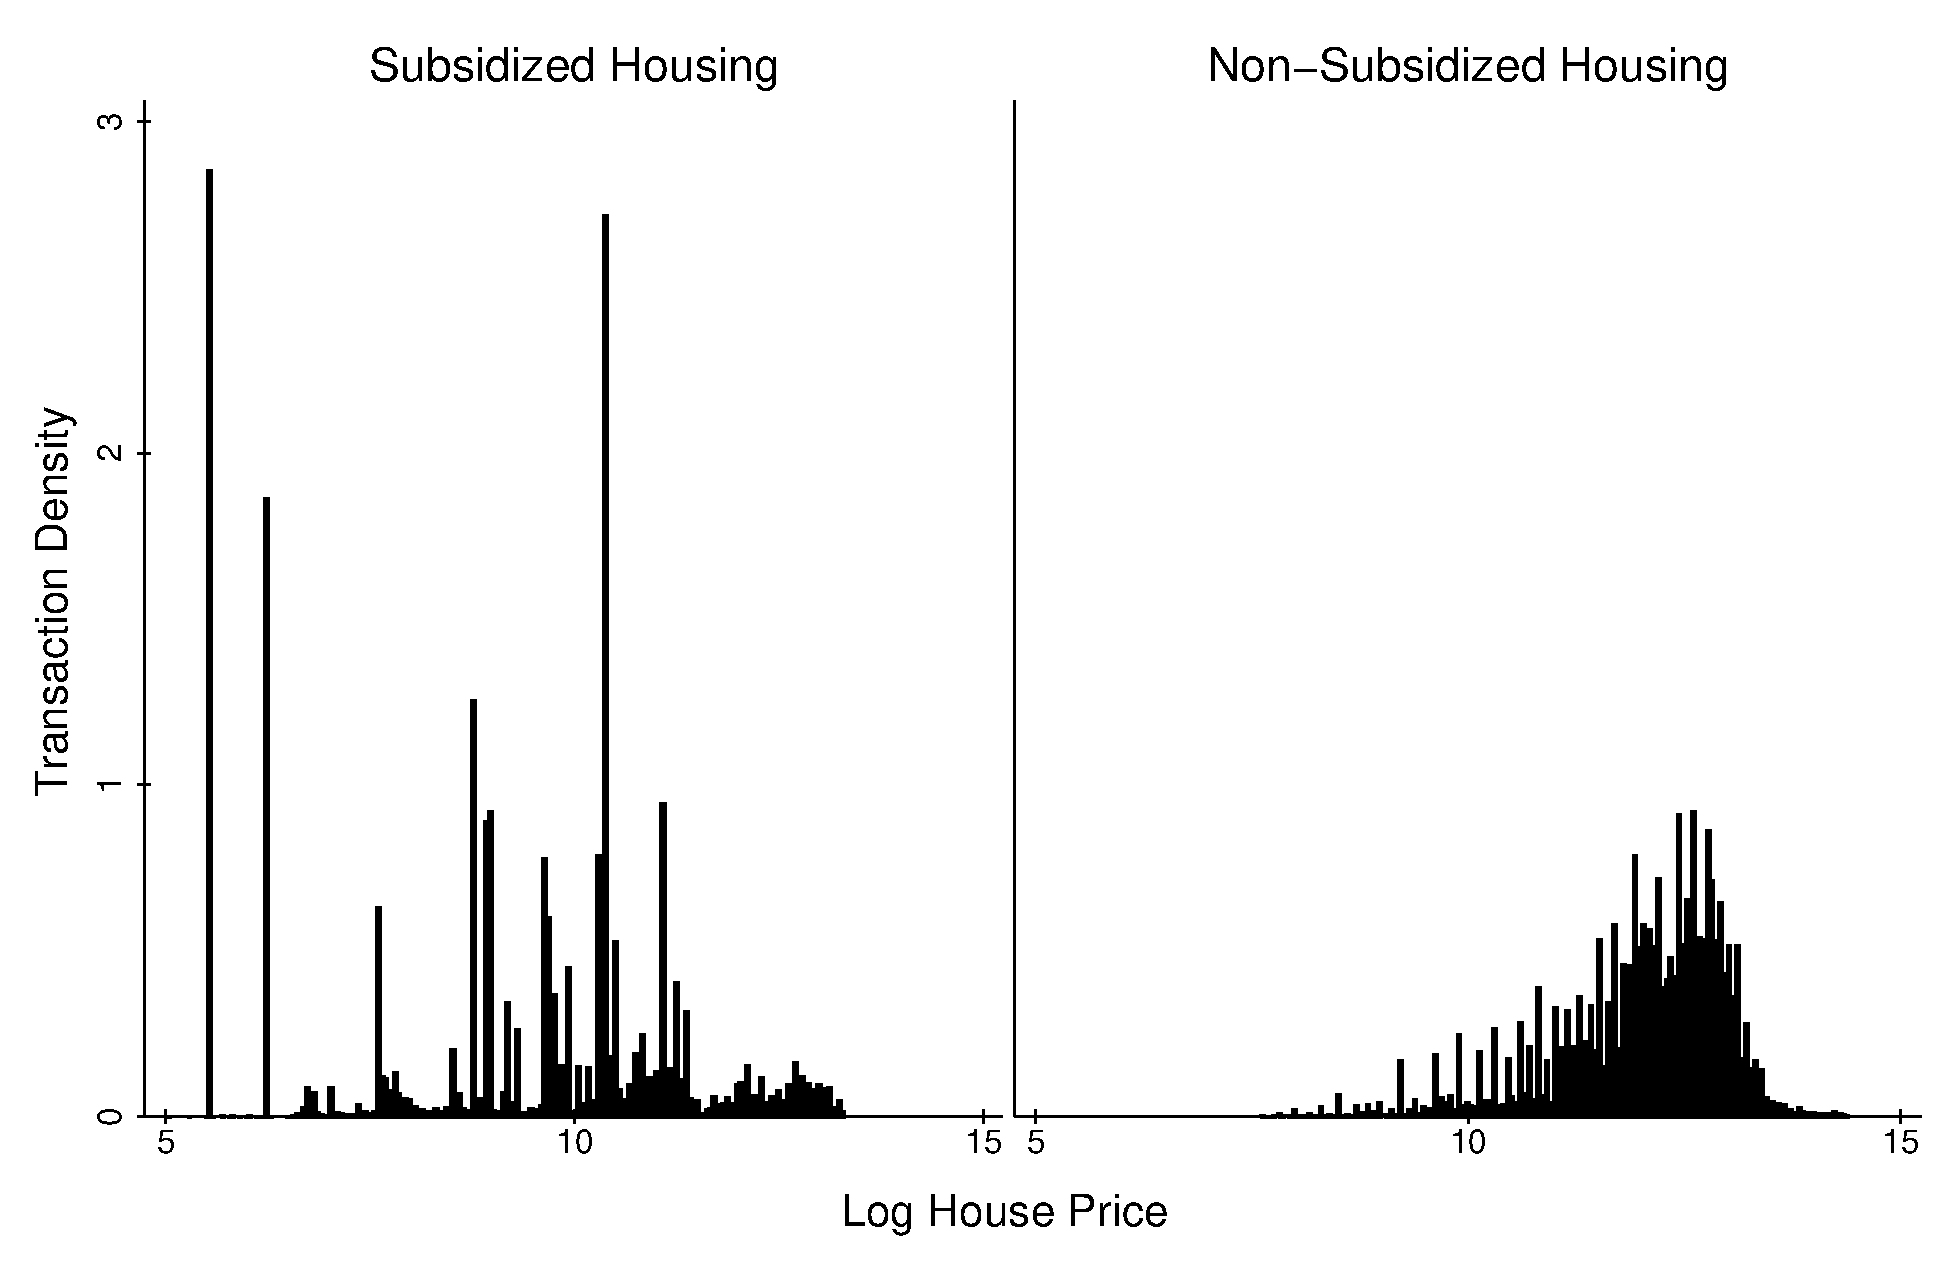
\includegraphics[scale=.4,trim={0cm 0cm -1cm 0cm}]{figures/summary_pricedist.pdf}}
%\\
%\footnotesize{Note: Transactions are censored at R100,000.}
\end{figure}

\begin{figure}[t!]
\centering
\caption{Housing Project Map}\label{figure:map}
\tcbox[colback=white,boxrule=.35mm,boxsep=0mm]{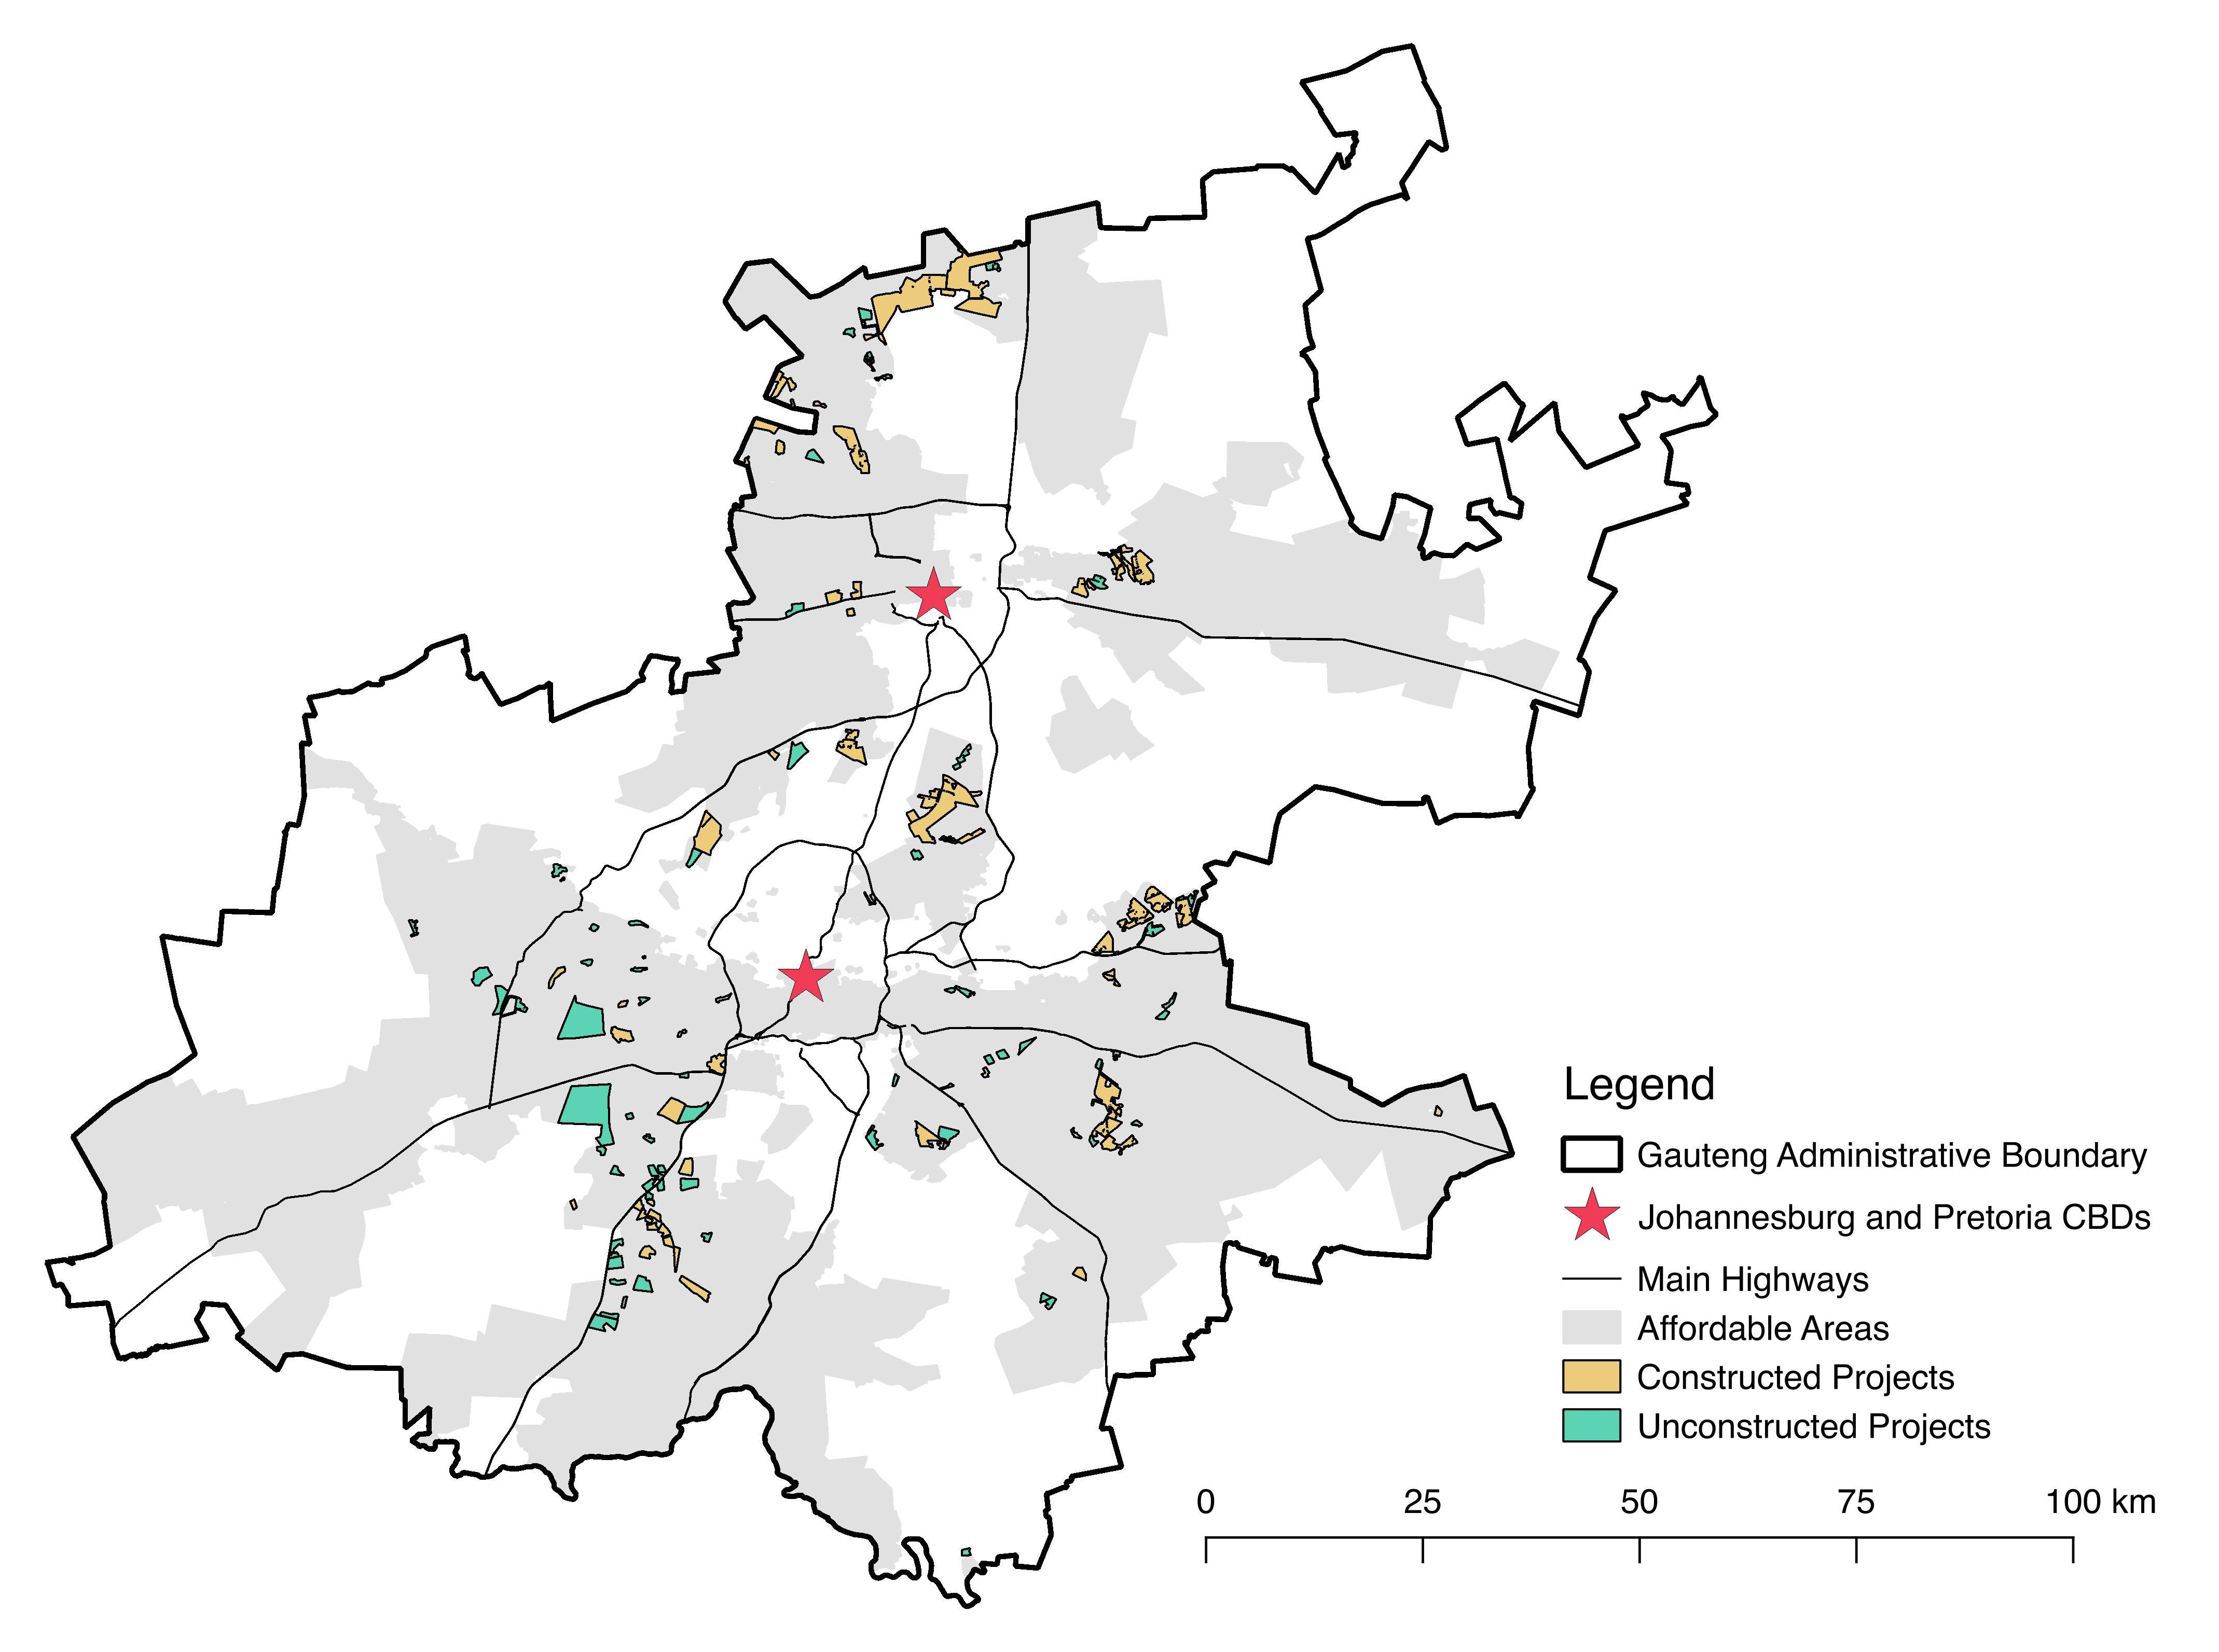
\includegraphics[scale=.132,trim={.9cm .4cm .9cm .4cm}]{figures/explanmap.jpg}}
\end{figure}

\subsubsection*{Planned but Unconstructed Housing Projects}

Identifying 57constructed housing projects leaves 99planned but possibly unconstructed housing projects in the administrative map.  We propose using these projects as counterfactuals, capturing the level of urban development that would have occurred in the absence of construction. Because our deeds data cover the 2001-2011 period and the policy maps pertain to 1994-2008, a concern is that some of the remaining 99 projects were planned and delivered prior to 2001. In order to determine which of the unconstructed projects were planned between 2001 and 2011, we make use of National Treasury budget reports.  We are able to digitize data for 132 projects from budget reports spanning 2004 to 2009, which detail the name, start date, expected completion date, and cost of each housing project.  We then use a string-matching algorithm to link project names from the budget reports to the administrative maps. This procedure results in a final sample of 60unconstructed projects. We provide further details about the digitization and string-matching algorithm in appendix Appendix~\ref{table:stringmatch}. Figure \ref{figure:map} shows the geographic setting of our analysis, where our final sample of constructed and unconstructed project boundaries are mapped out. Importantly, Figure \ref{figure:map} also shows that affordable areas, the coverage areas for our deeds data, contain every project boundary. While constructed and unconstructed projects are often adjacent to each other, possibly indicating cases where authorities were unable to complete final phases of planned projects, there are also many examples of isolated projects of both types.  Projects are generally located at relatively great distances from central business districts (CBDs), validating that vacant or inexpensive land plots are especially targeted by housing authorities.  Despite their distance from the CBDs, housing projects are often next to arterial highways easing commuting costs for recipients.


%We then use a fuzzy-string matching algorithm with bigrams to link project names from the budget reports to the administrative maps.  We keep all matches with over 60\% similarity, with 44 projects matching exactly.  Appendix~\ref{table:stringmatch} compares unmatched and matched projects finding that matched projects have much higher densities of informal housing and project housing density, but similar densities of formal housing and project dates.  One reason may be that the budget reports only include larger, more expansive projects. We find that the project start date (from the budget reports) is three years before the project completion date (from the deeds data) on average.  In other words, beneficiaries receive title to their new houses about three years after the housing program is announced in the budget.  Using this lag, we assign an expected completion date for unconstructed projects that is three years after the announced start-date in the budget reports.  Since the budget data does not include month of planning, we assign a random month for unconstructed projects, which ensures that this date is uncorrelated with seasonality but also introduces measurement error in the timing of unconstructed projects.  This error is only likely to affect the housing transaction estimates, which are the only estimates performed at the monthly level.  

%We use a limited definition of verified seller names to minimize the chances that unconstructed projects are misclassified as constructed projects.  However, this approach increases the possibility that this definition mistakenly excludes constructed projects.

\begin{table}[h!]
\centering
\caption{Project Descriptions}\label{table:projectdescriptions}
\vspace{-2mm}
\begin{tabular}{l*{1}{cc}}
\toprule
 &Constructed &Unconstructed  \\
\midrule
Proposed   &          5  &    20  \\
Planning   &          8  &    12  \\
Under Implementation& 12 &     4  \\
Complete   &          6  &     1  \\
No Description &       37  &    28  \\ 
Total  &  68  &     65  \\
\bottomrule
\end{tabular}
\end{table}

We note that our approach is not without limitations, and may introduce measurement error insofar as we are mis-attributing deeds to housing projects (false-positives), or wrongly assuming a project is unconstructed (false-negatives). To provide some validation for our classification, we tabulate in Table~\ref{table:projectdescriptions} project descriptions from the administrative policy maps according to whether projects are classified as constructed or unconstructed. We find that constructed projects are more likely to be classified as ``completed" or ``under implementation", while unconstructed projects are more likely to fall into ``proposed'' or ``planning'' categories.\footnote{We cannot verify that every project description, when available, is indicative of the most recent project status.}


\subsubsection*{Non-subsidized housing transactions}

To examine spillovers on nearby non-subsidized housing, we retain the remainder of properties that satisfy none of the criteria in the filtering procedure. We focus on properties located within 4 kilometers of constructed and unconstructed housing projects, forming a sample of over 140,000 transactions.  We exclude the top 1\% of prices as well as prices below 2,500 Rand, which are likely composed of mis-measured prices, or titles exchanged between family members. The price distribution of this sample is displayed in the right panel of Figure \ref{figure:transactionhist}, which stands in contrast to the distribution of subsidized transactions in the left panel. %In Figure \ref{figure:densitytime}, we plot monthly transaction densities around the modal transaction month for every constructed project, separating project transactions (upper panel) from non-project transactions (lower panel).

%\begin{figure}[t!]
%\centering
%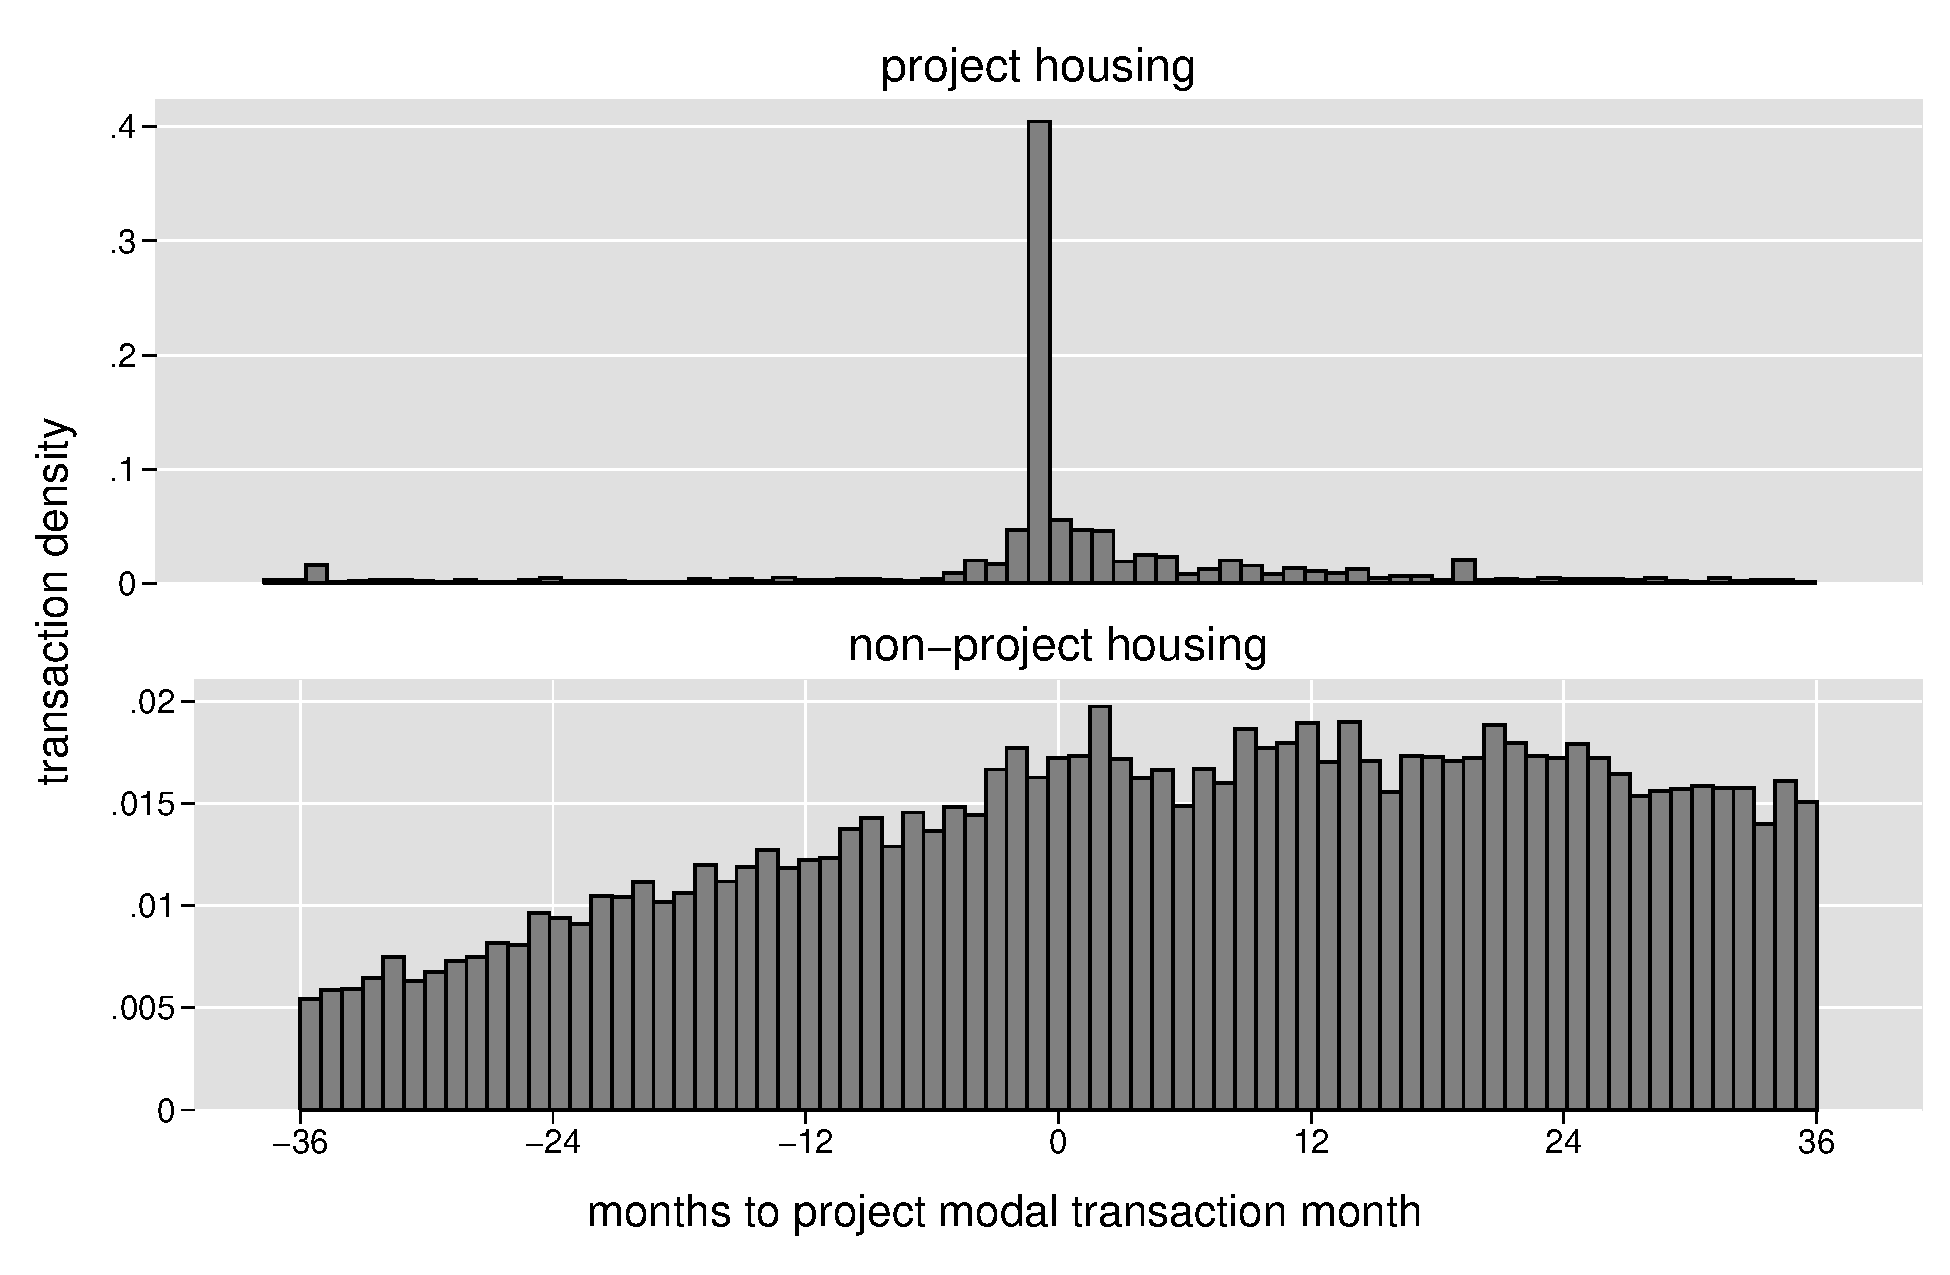
\includegraphics[scale=.4]{figures/summary_densitytime.pdf} 
%\caption{Transaction Densities Relative to Modal Project Month}\label{figure:densitytime}
%\end{figure}



%%%%%%%%%%%%%%%%%%%%%%%%%%%%%%%%%%%%%%%%%%%%%%%%%%
%%%%%%%%%%%%%%%%%%%%%%%%%%%%%%%%%%%%%%%%%%%%%%%%%%
%%%%%%%%%%%%%%%%%%%%%%%%%%%%%%%%%%%%%%%%%%%%%%%%%%

%Descriptive evidence supports our project definition in several ways.  First, Figure~\ref{figure:topfivesellers} shows that the top five most frequently occurring seller names clearly correspond to government housing programs in the region.  Second, transaction prices for project houses are strongly clustered around subsidy values.  Figure~\ref{figure:transactionhist} provides a histogram of deed prices under R100,000 for transactions that meet our project definition as well as those that do not.  Government agencies often record either zero price or the value of the subsidy in the deeds, producing substantial bunching at these values compared to non-project transactions.  At the same time, there exists a small density of projects smoothly distributed across the lower range of prices for project housing, which may be evidence of some misclassification of our project housing measure.


%We assign a completion date for each project according to the modal year of these deeds transactions.  Figure~\ref{figure:densitytime} indicates the distribution of transaction dates for properties within a 4 km buffer around housing projects (above panel) and within the selected project areas (below panel).  Project areas exhibit substantial bunching during a single month when projects were completed.  There are also more transactions after the modal year than before the modal year, consistent with either a gradual roll-out for some project areas or immediate resale of projects houses after construction, which would be counter to housing regulations.  
%We then include only clusters where over 50\% of transactions occur during the modal year, which excludes half of total clusters.  This approach helps to exclude incremental projects as well as possible land titling programs, allowing us to leverage the sharp timing of large project construction in our identification.  

%Evidence of similar bunching around the modal year for transactions coded as non-project transactions (above panel) would suggest that we may be miscoding project transactions as non-project transactions; instead, we find a smooth pattern relative to the modal year for these non-project transactions.  The slight increase in density around and just following the modal year may also be consistent with housing projects having an immediate impact on local housing markets, which we will explore further below.

%To measure formal housing market impacts, we analyze over 500,000 housing transactions from the South African National Deeds Office covering the universe of transactions for suburbs in the bottom 20\% of the housing market between 2003 and 2011 in the Gauteng Province (including the Johannesburg metro area).  The bottom 20\% suburbs were selected relative to prices in 2003 and followed every year from 2003 to 2011.  These data were provided by the Affordable Land and Housing Data Centre (ALHDC), which tracks affordable housing markets.\footnote{the ALHDC is an initiative launched by the Centre for Affordable Housing Finance in Africa, an independent think tank. }  These data include the price, exact location, plot size, buyer name, and seller name for each transaction.  To isolate spillover effects, we focus on transactions occurring within 4 kilometers of a housing project.  Finally, we exclude the top 1\% of prices as well as prices below 2,500 Rand, which are likely composed of measurement error or exchanging of titles between family members.

\subsection{Census Data}

To measure impacts on dwelling characteristics, we use the 2001 and 2011 national censuses of population and housing. Specifically, we analyze household-level responses describing the quality of their living quarters. Our outcomes are mainly binary indicators, and pertain to the household's access to services (flush toilets, water tap, electricity access), housing durability, and tenure arrangements. We identify households at the {\it small-area} level, the smallest available census geography. The province of Gauteng is divided between approximately 11,000 small areas in 2001, and 17,000 small areas in 2011.\footnote{Despite many boundaries being very similar, census geographies are not constant in both time periods. Most of the 2001-2011 growth in census small areas is due to geographies being split into more part in the 2011 census.} On average, each census area contains 170 household. Though we observe responses from every surveyed household in both census waves, the data does not allow to link households across time periods. 

\begin{figure*}[t!]
        \centering
        \caption[ Building-Based Land Use Data ]
        {\small Building-Based Land Use Data } 
        \vspace{2mm}
        \begin{subfigure}[b]{0.48\textwidth}
            \centering
            \frame{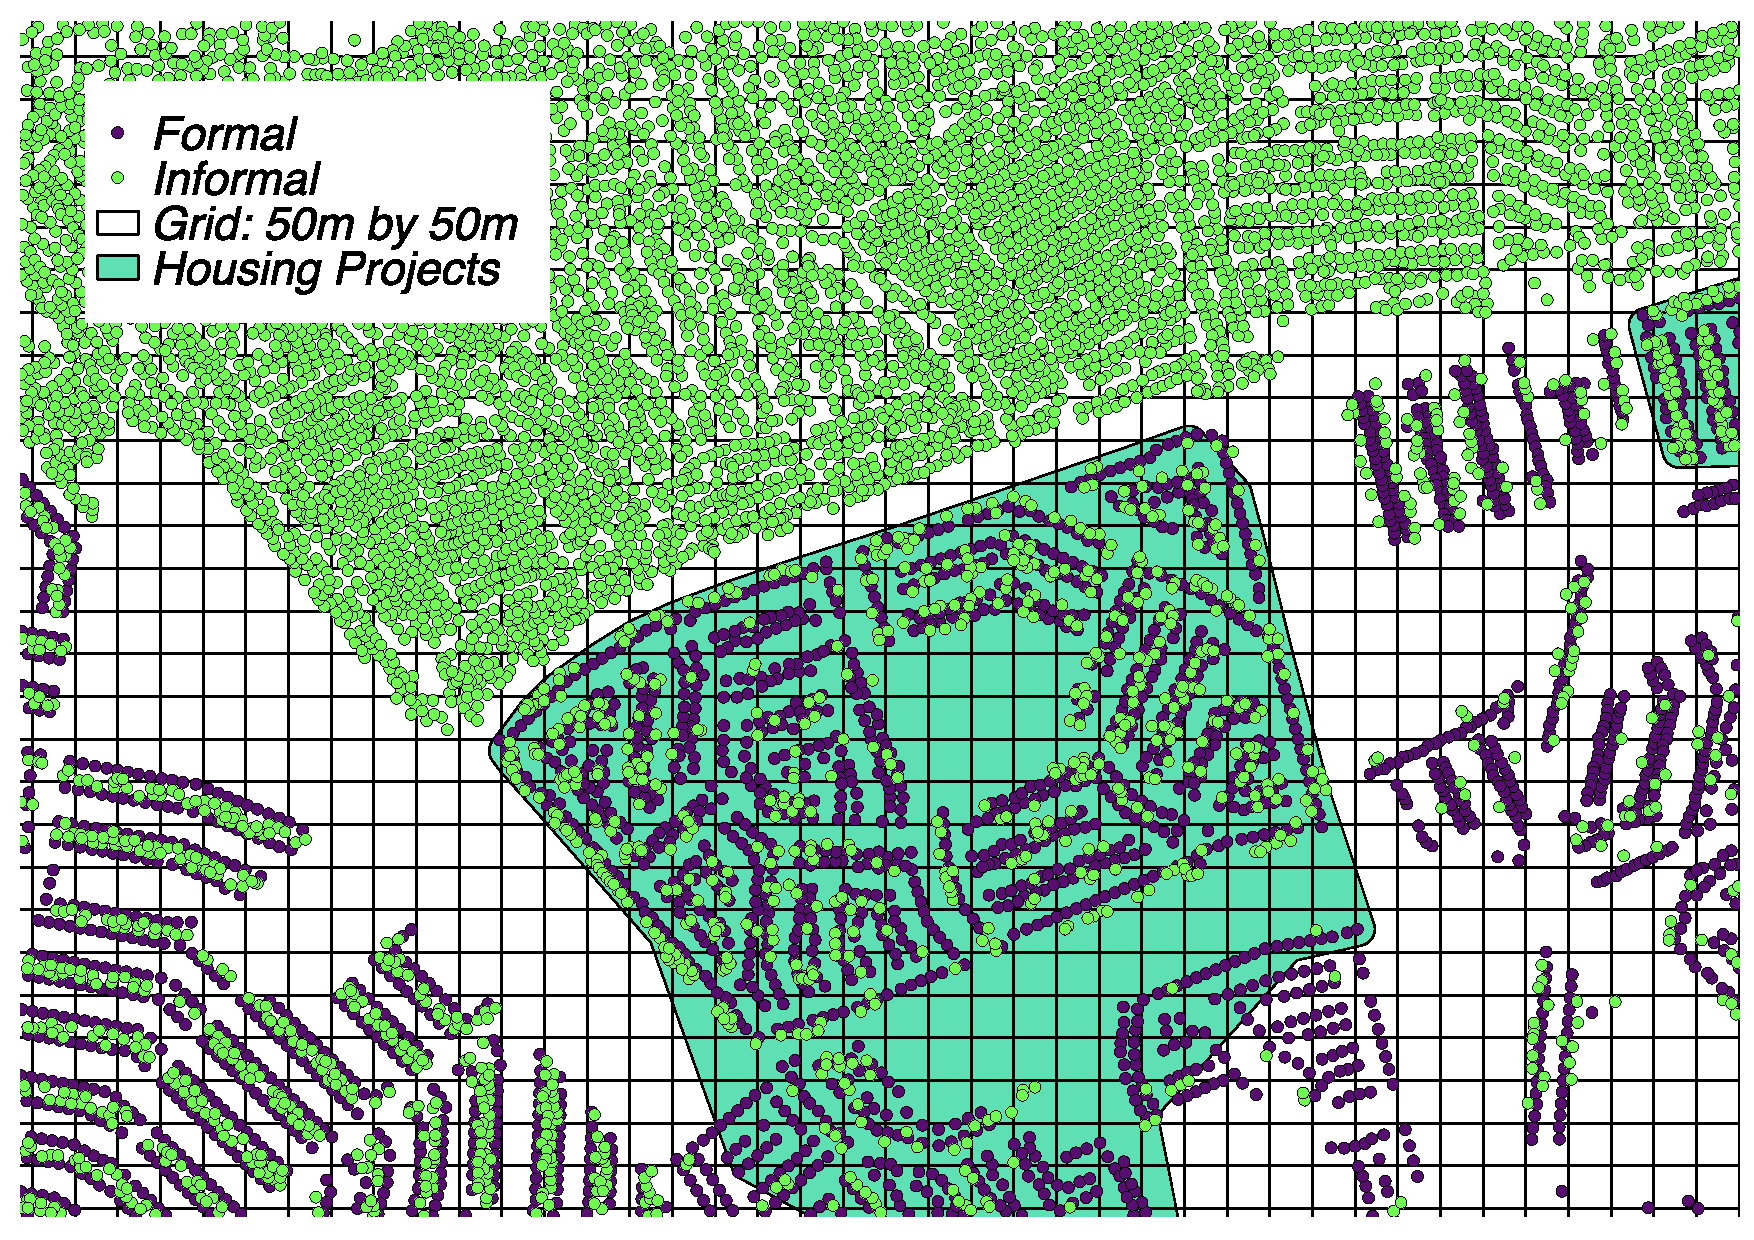
\includegraphics[width=\textwidth,trim={0cm 0cm 0cm 0cm}]{figures/bblu_map.jpg}}
            \caption[Network2]%
            {{\small raw data identifying (in)formal structures}}    
            \label{fig:prefor}
        \end{subfigure}
        \hfill\quad
        \begin{subfigure}[b]{0.48\textwidth}  
            \centering 
            \frame{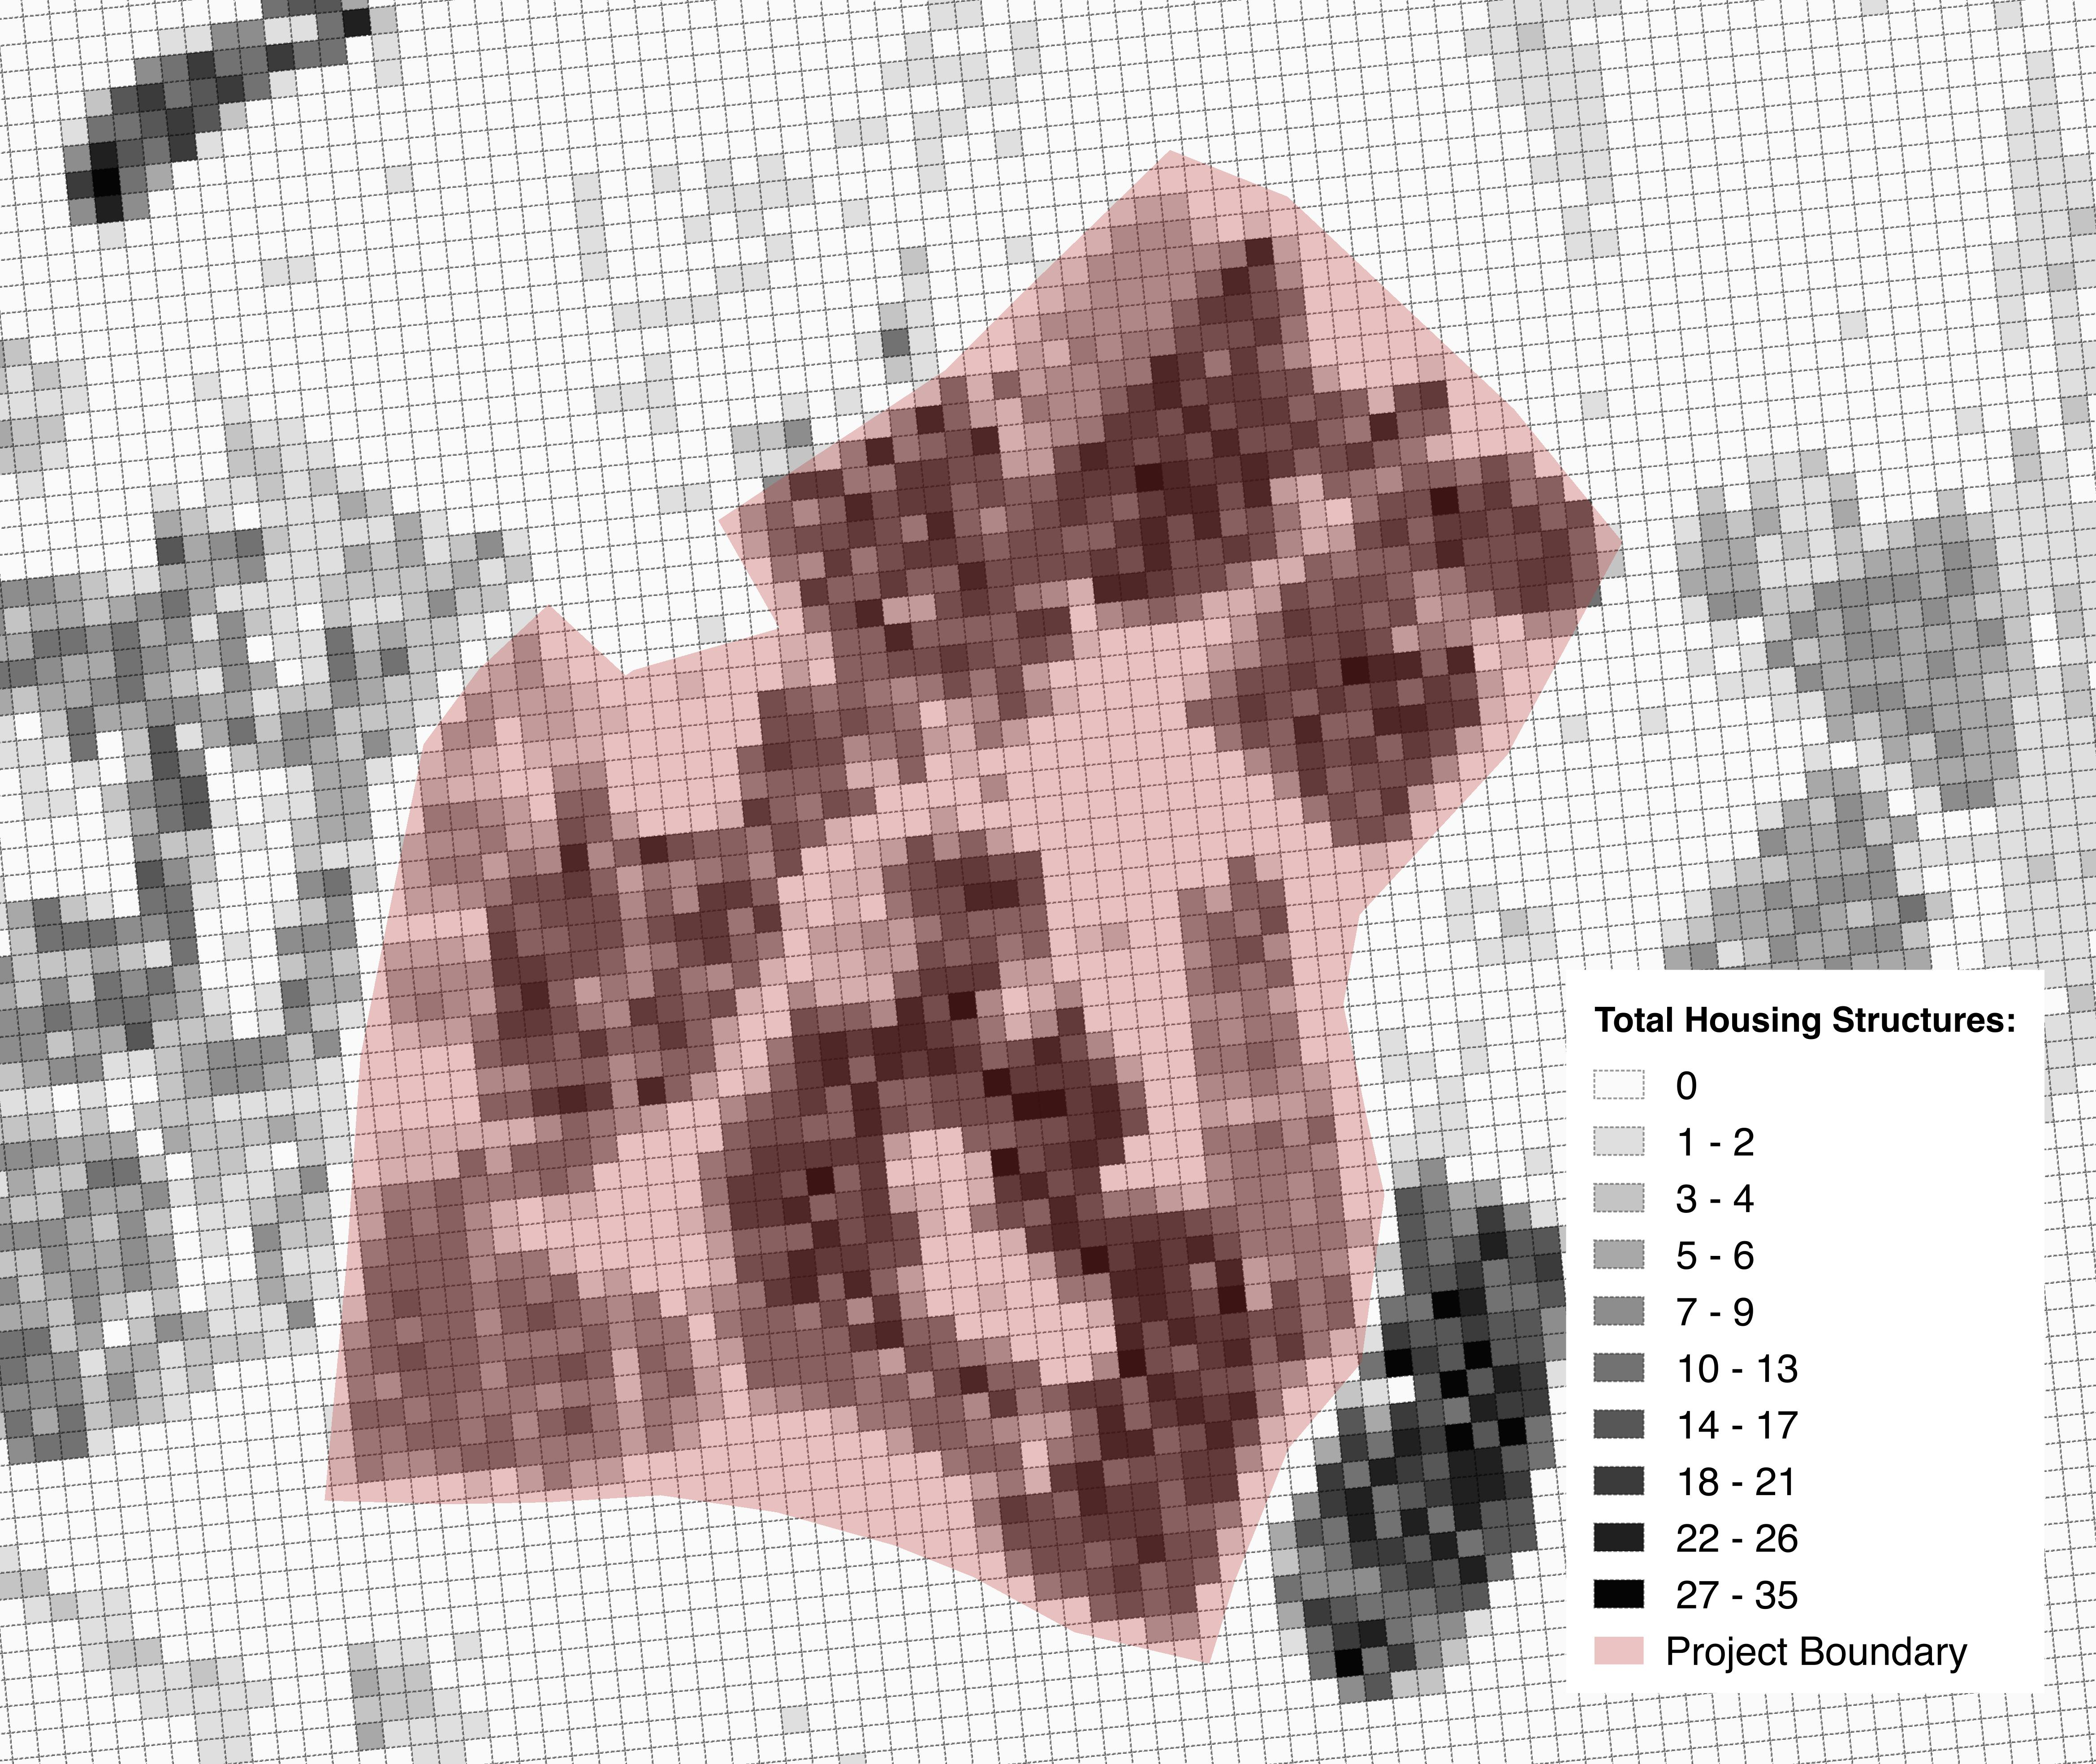
\includegraphics[width=\textwidth,trim={0cm 0cm 0cm 0cm}]{figures/bblu_grid.jpg}}
            \caption[]%
            {{\small 50m$\times$50m grid cells data aggregation}}    
            \label{fig:preinf}
        \end{subfigure}
        \label{fig:bblumaps}
    \end{figure*} 

\subsection{Building Based Land Use}

Our final data source consists of hand-coded building surveys derived from high-resolution aerial and satellite imagery. We obtain these data from GeoTerraImage (Pty) ltd., a local remote-sensing specialist. The data differentiates structures within over 30 categories, including formal and informal residential dwellings. Informal housing structures are easily identified from their temporary nature, often made of materials such as recycled wood and corrugated metal. In contrast, formal housing structures are permanent, generally made out of brick, and may have a pitched or a flat roof with tiles, zinc panels, or other materials. Importantly for our analysis, the data encodes backyard shacks as informal structures, but allows to distinguish between backyard and other types of informal buildings. We track changes in residential development by using all two available survey waves in Gauteng: 2001 and 2012. As a validation exercise, we compute aggregated building counts at the census small-area level, and check the resulting figures against the number of households reporting to live in formal/informal housing in the census. The two data sources paint a consistent picture of housing in Gauteng, with highly correlated ($\geq$ 0.85) formal and informal building quantities in both available comparison years.\footnote{We correlate the 2001 and 2012 building surveys with the 2001 and 2011 censuses, respectively.} For estimation purposes, we transform this data into 50m$\times$50m grid cells aggregates, thereby creating five measures of housing density and the built environment: total residential structures, formal residential structures, informal residential structures, backyard informal and non-backyard informal structures.\footnote{Total housing is the sum of formal and informal housing, while informal  } These grid cells will be the main units of observations for our housing density regressions, described in section \ref{WUT}. In Figure \ref{fig:bblumaps}, we provide an example of the raw data and a depiction of our griding procedure, using the 2012 data wave.



%as well as the yearly General Household Survey for 2005 through 2014.  

% The General Household Survey includes additional details on participation in housing programs over time for a random sample of around 35,000 households in the Gauteng Province. 
% Both surveys include information about dwelling type, employment, income, and demographics for each household.  The General Household Survey includes additional details on participation in housing programs over time for a random sample of around 35,000 households in the Gauteng Province.

%\subsection{Constructed Housing Projects}

%We construct our primary measure of housing projects by matching a set of known characteristics for housing projects for properties transacted in the deeds data.  This procedure results in spatially distinct clusters that form the definition of housing projects for the empirical analysis (\cite{serihistory}).  Due to data limitations, we are not able to differentiate between greenfield and in-situ upgrading projects in the analysis.

%\subsubsection{Seller Identity}
% prob yes and large : 2770 / 127600 = 2\%

%\subsection{Planned but Unconstructed Housing Projects}

%The administrative spatial data identifies many project areas that do not appear to have received housing projects, as measured by having fewer than 5 housing project transactions per square kilometer.  We use these areas to create a sample of planned but unconstructed housing projects to serve as counterfactuals areas in our analysis.

%Identifying 57constructed housing projects leaves 99planned but possibly unconstructed housing projects in the administrative map.  We propose using these projects as counterfactuals, capturing the level of the development that would have occurred in the absence of full construction.  

%In order to determine which of the unconstructed projects were planned to be completed between 2001 and 2011, we construct an estimated completion date using National Treasury budget reports.  We were able to digitize data for 132 projects from budget reports spanning 2004 to 2009, which detail the name, start date, expected completion date, and cost of each housing project.  We then use a fuzzy-string matching algorithm with bigrams to link project names from the budget reports to the administrative maps.  We keep all matches with over 60\% similarity with 44 projects matching exactly.  Appendix~\ref{table:stringmatch} compares unmatched and matched projects finding that matched projects have much higher densities of informal housing and project housing density, but similar densities of formal housing and project dates.  One reason may be that the budget reports only include larger, more expensive projects.

%We find that the project start date (from the budget reports) is three years before the project completion date (from the deeds data) on average.  In other words, beneficiaries receive title to their new houses about three years after the housing program is announced in the budget.  Using this lag, we assign an expected completion date for unconstructed projects that is three years after the announced start-date in the budget reports.  Since the budget data does not include month of planning, we assign a random month for unconstructed projects, which ensures that this date is uncorrelated with seasonality but also introduces measurement error in the timing of unconstructed projects.  This error is only likely to affect the housing transaction estimates, which are the only estimates performed at the monthly level.  This procedure results in a final sample of 60unconstructed projects.

%Table~\ref{table:projectdescriptions} tabulates project descriptions from the administrative data according to our definitions of completed and uncompleted.  We find that constructed projects are much more likely to be classified as ``completed,'' ``planning,'' or in ``implementation'' while unconstructed projects are more likely to fall into ``Uncertain'' or ``Investigating'' categories.  These correlations provide an external validation of our classification of constructed and unconstructed projects with deeds records.

\section{Empirical Methodology}\label{section:methodology}

To ascertain the urban development impacts of subsidized housing both within project boundaries as well as nearby, we implement a difference-in-differences strategy assessing changes in outcomes for constructed projects, using unconstructed projects as counterfactuals. Given the varying temporal and spatial granularity of our measured outcomes, we estimate different forms of the following specification:

\begin{equation}
y_{ipt} \, = \, \lambda_p + \sum\limits_{d} I^d_{ipt}\Big( \alpha^d D_{pt}C_{p} \, + \, \beta^dD_{pt} \, + \, \gamma^dC_{p} \, + \, \theta^{pt} \Big) \, + \, \delta X_{ipt} \, + \, \varepsilon_{ipt}
\end{equation}

\noindent where $y_{ipt}$ is the outcome for unit $i$ in vicinity of constructed/unconstructed project $p$ observed at time $t$. $D_{pt}$ and $C_{p}$ are the usual post and treatment dummies, where $D_{pt}$ equals one if period $t$ is after project $p$ was constructed, and $C_{p}$ equals one if project $p$ is constructed. We interact the standard DiD set-up with a set of distance dummies $I^d_{ipt}$, where $I^d_{ipt}$ equals one if unit $i$ is located at distance $d$ from project $p$'s boundary. This specification also admits project fixed-effects $\lambda_p$, a vector $X_{ipt}$ of additional control variables, and idiosyncratic error $\varepsilon_{ipt}$. As will be clear from sections \ref{lol} and \ref{lol}, distances $d$ are defined to account for impacts both inside and outside of project boundaries. This set-up thus allows for effects to vary flexibly according to location.

We interpret the coefficients of interest $\alpha^d$ as the causal impact of subsidized housing on outcome $y$, at distance $d$ of a project boundary. Specifically, $\alpha^d$ measures the differential change in outcomes for constructed projects, relative to unconstructed projects. A causal interpretation assumes that absent of any housing policy, constructed and unconstructed project areas would experience similar dynamics in terms of residualized outcomes. 

\section{Descriptive Statistics}\label{section:descriptives}

%To assess the extent to which our definitions accurately measure housing projects, Figure~\ref{figure:gcrooverlap} maps our cluster definitions on top of administrative data on housing projects.  We see strong overlap between clusters and administrative projects, providing additional support for our deeds-based cluster measure.  A few smaller clusters do not overlap with administrative definitions, which is consistent with the administrative data recording larger, higher-cost projects.  Similarly, administrative boundaries that do not contain clusters are likely to be projects that were planned but were not completed or are scheduled to be completed in the future.

% \begin{figure}
% \caption{Clusters and Administrative Project Boundaries}\label{figure:gcrooverlap}
% \centering
% 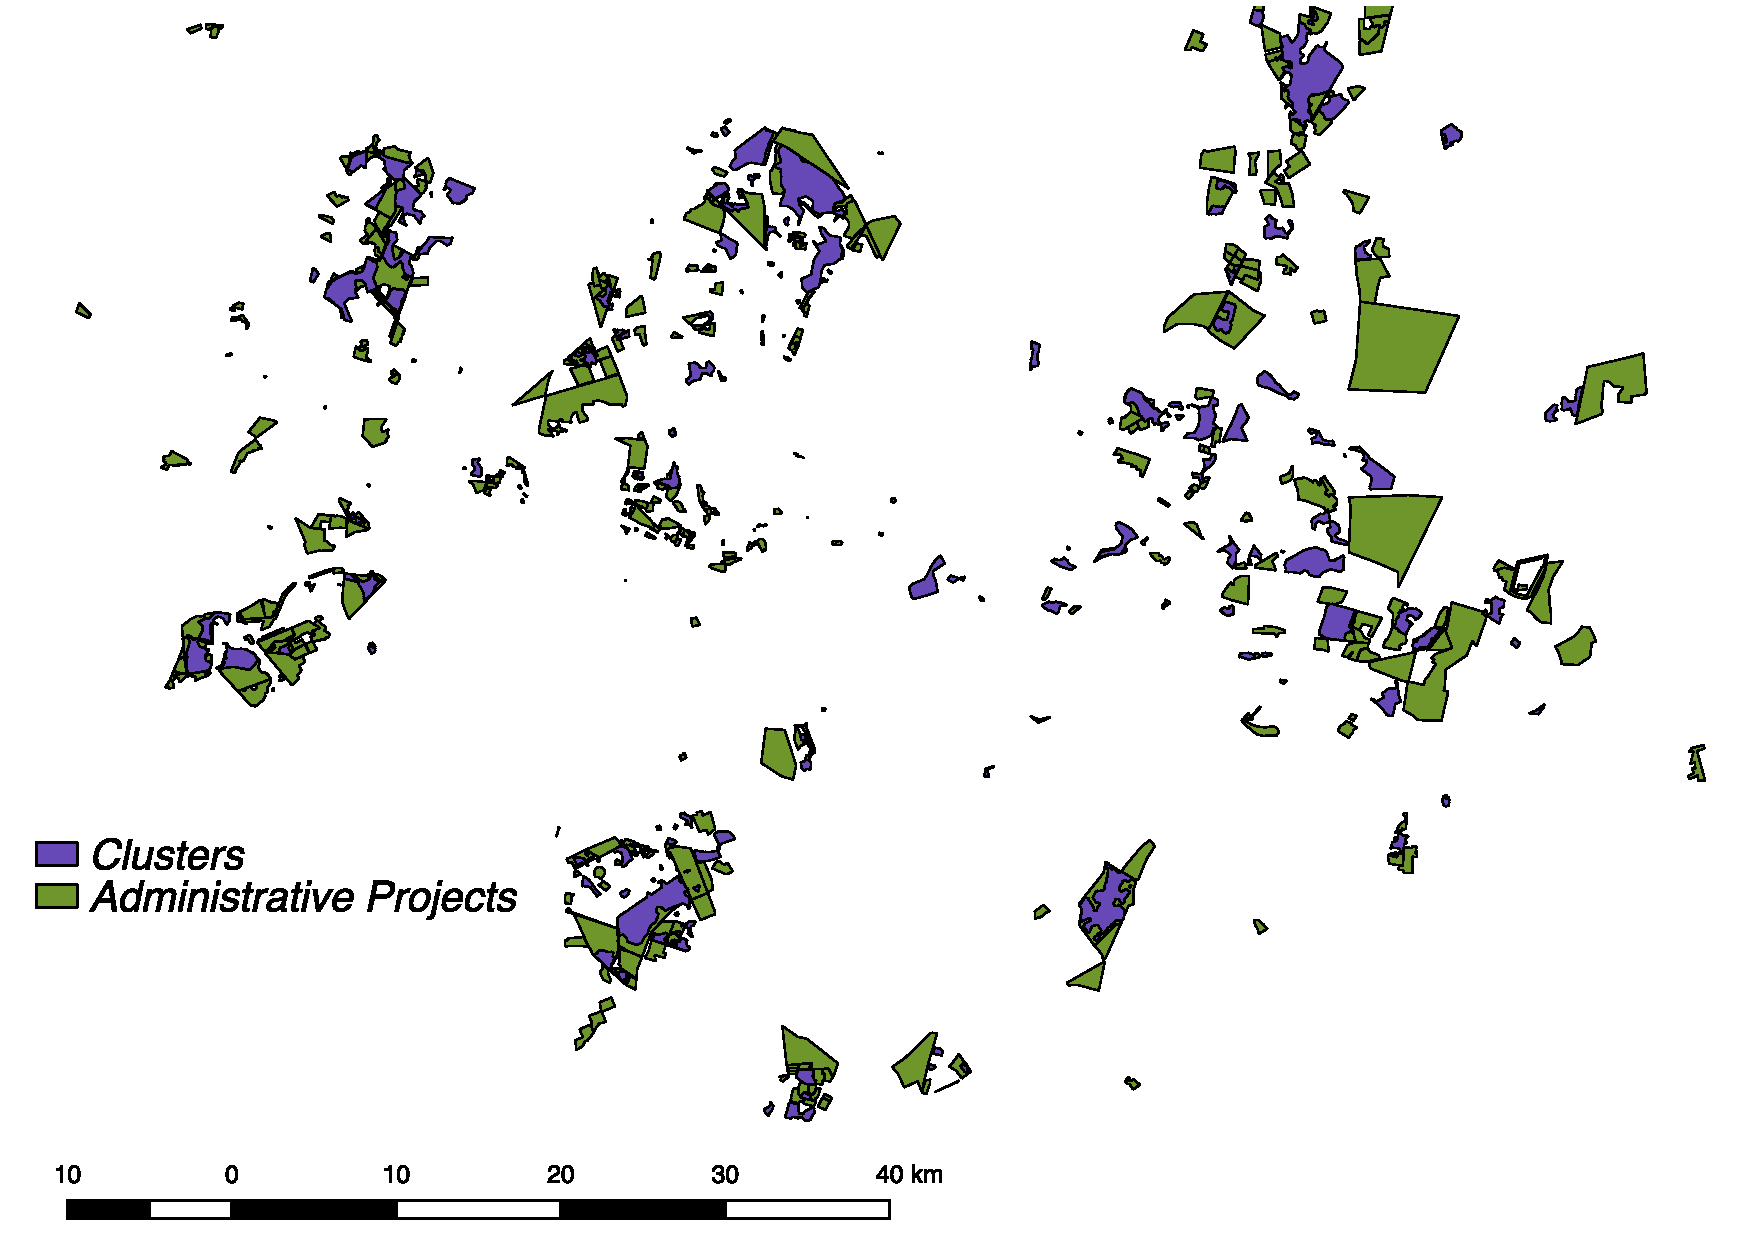
\includegraphics[scale=.5]{figures/gcro_convexhull_overlap.pdf} \\
% This figure includes the northern half of housing projects.
% \end{figure}

To contextualize our main analysis, we first provide descriptive evidence on the location, size, and housing stock of areas surrounding our sampled projects. Table~\ref{table:projectdescriptives} reveals that the policy provides substantial quantities of housing, delivering on average upwards of 850 new units per project. Constructed projects are larger in area than unconstructed projects, likely due to some unconstructed project representing smaller extensions to previously implemented projects.

givesprovides descriptive statistics at baseline for our sample of 57constructed and 60unconstructed projects.    These differences are also exacerbated by a few very large constructed projects.  Compared to unconstructed projects at baseline, constructed projects have smaller densities of informal housing and slightly larger densities of formal housing, indicating better housing stock on average.  At the same time, deeds records indicate somewhat higher house prices for homes in unconstructed areas.  Both types of projects share similarly long distances to Central Business Districts consistent with authorities targeting inexpensive, vacant land for these projects.  With an average of around 500 project houses per square kilometer, these housing programs have the potential to strongly impact the local housing stock for constructed project areas, in many cases doubling the existing stock of formal housing.

% Figure~\ref{figure:map} maps our sample of unconstructed and constructed housing projects.  We find that projects fall exclusively within affordable housing areas (defined as enumerator areas in the bottom quintile of house prices in 2003).  While constructed and unconstructed projects are often adjacent to each other possibly indicating cases where authorities were unable to complete final phases of planned projects, there are also many examples of stand-alone projects of both types.  Projects are generally located at relatively great distances from central business districts (CBDs), which suggests that vacant or inexpensive land plots are especially targeted by housing authorities.  Despite their distance from the CBDs, housing projects are often next to arterial highways easing commuting costs for recipients.

\begin{table}[t!]
\centering
\caption{Housing Projects at Baseline}\label{table:projectdescriptives}
\vspace{-2mm}
\begin{tabular}{l*{1}{cc}}
\toprule
  &Constructed &Unconstructed \\
\midrule
Number of Projects  &       68 &       65 \\
Area (km2) &       3.61 &       2.21  \\
Delivered Houses  &     858.75 & .      \\
House Price within 1km (Rands) &   215,172.77   &   204,490.48   \\
Distance to CBD* (km) &  30.38  &     32.92   \\
\bottomrule
\multicolumn{3}{l}{\footnotesize *measured with respect to Johannesburg and Pretoria. }
\end{tabular}
\end{table}

\begin{table}[b!]
	\centering
	\caption{Infrastructure and Demographics at Baseline}\label{table:projectdescriptivescensus}
\vspace{-2mm}
\begin{tabular}{l*{1}{ccc}}
\toprule
& Constructed & Unconstructed & All Households \\
\midrule
Flush Toilet&0.55&0.45&0.81 \\
Piped Water in Home&0.13&0.19&0.46 \\
Electricity for Cooking&0.32&0.37&0.72 \\
Electricity for Heating&0.29&0.35&0.70 \\
Electricity for Lighting&0.56&0.45&0.81 \\
Number of Rooms&2.74&2.49&3.57 \\
Household Size&3.43&3.19&3.19 \\
N&        196,467&         61,530&      2,344,122 \\
 
\bottomrule
\end{tabular}
\end{table}




Areas within 4 km of housing projects have greater total building density and higher ratios of  formal housing to informal housing compared to both the unconstructed and constructed projects.  Similarly, housing prices are much higher for properties outside of project areas.  These findings suggest that at similar distances away from central business districts, governments are still selecting less developed and less valuable land for housing projects.  At least in terms of building composition, density, and value, unconstructed projects seem to provide a better comparison group for constructed projects than simply examining nearby areas.  

\begin{figure*}[t!]
        \centering
        \caption[ Housing Densities in Constructed and Unconstructed Projects Areas ]
        {\small Housing Densities in Constructed and Unconstructed projects } 
        \vspace{2mm}
        \begin{subfigure}[b]{0.48\textwidth}
            \centering
            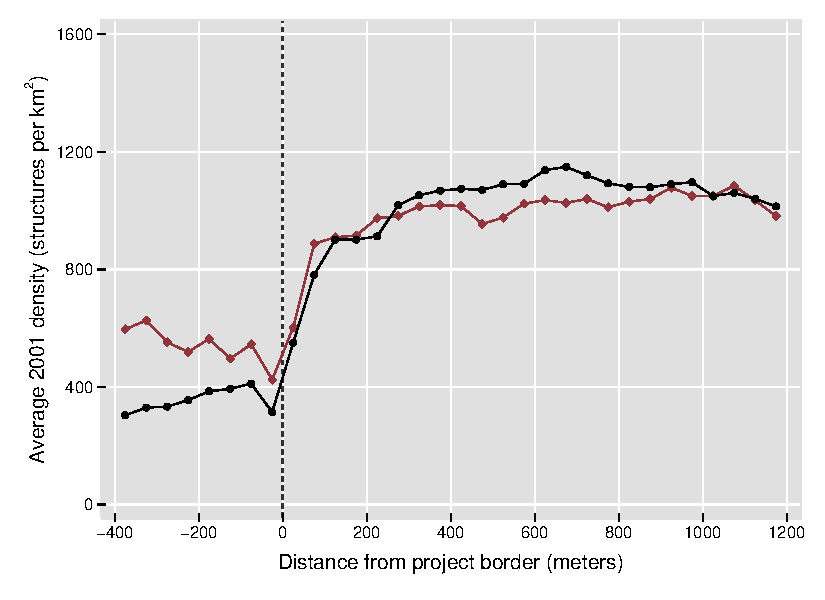
\includegraphics[width=\textwidth,trim={0cm .3cm 0cm 0cm}]{figures/bblu_for_pre_means}
            \caption[Network2]%
            {{\small pre-period formal housing density}}    
            \label{fig:prefor}
        \end{subfigure}
        \hfill
        \begin{subfigure}[b]{0.48\textwidth}  
            \centering 
            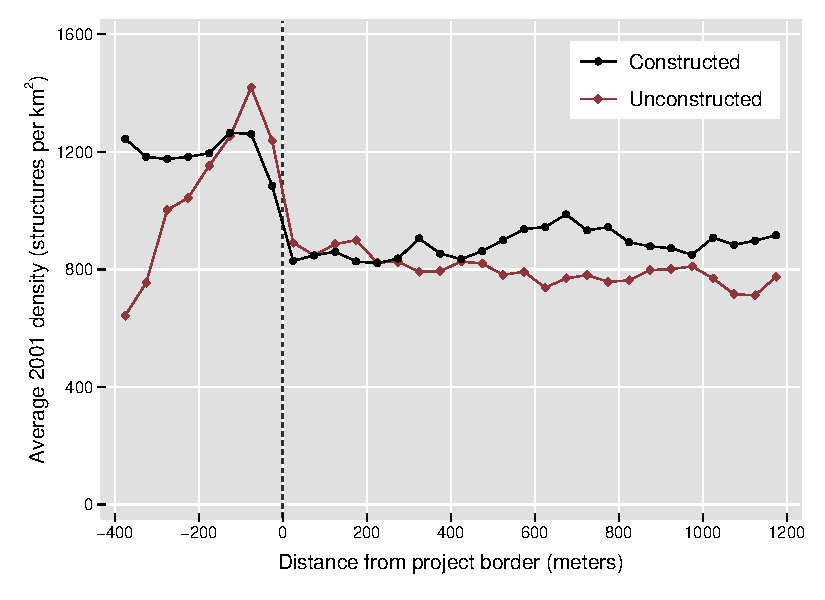
\includegraphics[width=\textwidth,trim={0cm .3cm 0cm 0cm}]{figures/bblu_inf_pre_means}
            \caption[]%
            {{\small pre-period informal housing density}}    
            \label{fig:preinf}
        \end{subfigure}
        \vskip 3mm \vskip 0pt
        \begin{subfigure}[b]{0.48\textwidth}   
            \centering 
            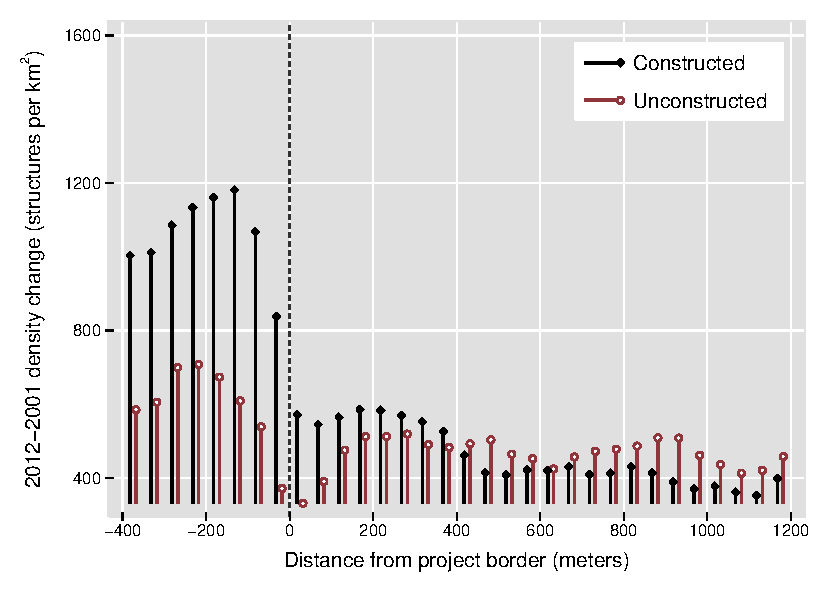
\includegraphics[width=\textwidth,trim={0cm .3cm 0cm 0cm}]{figures/bblu_for_rawchanges}
            \caption[]%
            {{\small formal housing density change}}    
            \label{fig:forchange}
        \end{subfigure}
        \hfill
        \begin{subfigure}[b]{0.48\textwidth}   
            \centering 
            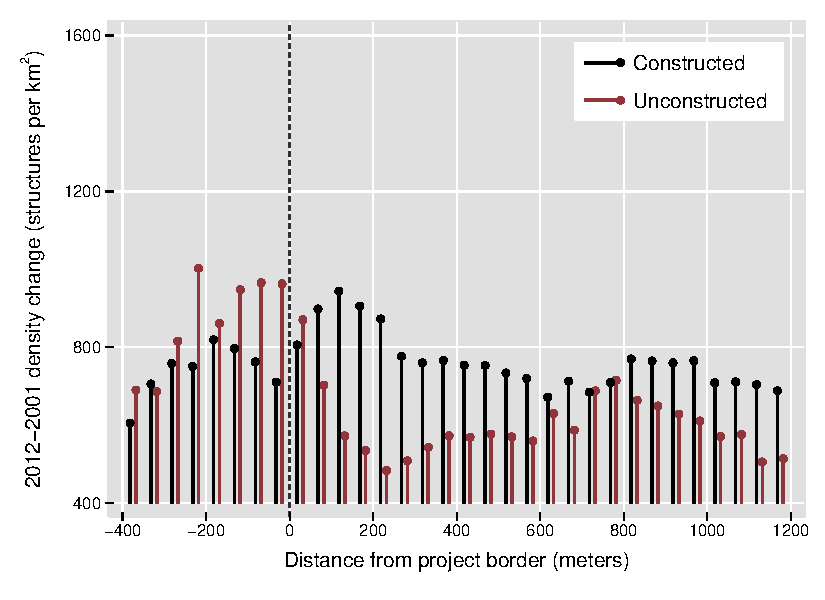
\includegraphics[width=\textwidth,trim={0cm .3cm 0cm 0cm}]{figures/bblu_inf_rawchanges}
            \caption[]%
            {{\small informal housing density change}}    
            \label{fig:infchange}
        \end{subfigure}
        \label{fig:rawbblumeans}
    \end{figure*} 


Table~\ref{table:projectdescriptivescensus} compares census measures at baseline across constructed and unconstructed projects as well as areas within 4 km of housing projects.  We identify census block as pertaining to a housing project if over 30\% of their land areas overlap, which results in     15,454intersecting census blocks.  We find that unconstructed project areas lag behind constructed project areas across all demographic measures.  At the same time, constructed project areas are almost indistinguishable from nearby, non-project areas despite having fewer structures and greater population densities.

Taken together, these findings are consistent with governments (1) selecting low-cost land to implement projects and (2) facing high costs of finishing projects in dense slums.  These types of selection are important to consider when interpreting our results and to help motivate the difference-in-differences empirical strategy detailed below.



\section{Estimation Results}\label{section:results}

To estimate the impacts of housing projects both within their project areas as well as just nearby, we use a difference-in-differences strategy comparing changes in outcomes for constructed project areas to unconstructed project areas.  Given the varying spatial and temporal dimensions of the outcome measures, we use slightly different specifications of the difference-in-differences approach for each dataset.

\subsection{Infrastructure and Demographic Effects}\label{section:resultscensus}

To estimate impacts for census measures, we implement the following estimating equation, which estimates a standard difference-in-differences model both within the project area and just around the project area:
\begin{equation*}
y_{hpt} \, = \, \lambda_p + \sum\limits_{e} I^e_{hpt}\Big( \alpha^e D_tC_p \, + \, \beta^eD_t \, + \, \gamma^eC_p \, + \, \theta^e \Big) \, + \, \varepsilon_{hpt}
\end{equation*}
$y_{hpt}$ measures the outcome for household $h$ living in the vicinity of project $p$, observed in census year $t$.  $I^e_{hpt}$=1 if household $h$ is in the exposure area $e$ of project $p$.  Exposure area $e$ includes (1) project areas defined as census blocks that overlap over 30\% of their area with a housing project and (2) spillover areas defined as census blocks with fewer than 30\% area of overlap but whose centroids still fall within 1.5 km of the project boundary.  Appendix Figure~\ref{figure:bufferdesigncensus} maps an example of the project and spillover definitions.  The summation includes a standard difference-in-differences specification for each exposure area where $D_{t}\,\,$=1 if year $t$ is census year 2011 (post period) and $C_{p}\,\,$=1 if project $p$ has been constructed.  $\lambda_p$ includes a project fixed-effect to control for fixed differences between project areas that may be correlated with local demographic changes.  

The coefficients of interest are $\alpha^e$, which measure the differential change in outcomes for constructed relative to unconstructed projects (either in the project or spillover areas).  Interpreting this ceofficient as the causal effect of housing projects requires assuming that the areas within and nearby constructed projects would have evolved in the same way as corresponding areas for unconstructed projects in the absence of the program.  Descriptive evidence from Section~\ref{section:descriptives} indicates differences between constructed and unconstructed projects at baseline, particularly in terms of census measures.  These differences would likely bias any cross-sectional comparisons between projects. 

One potential concern is that whether a project is ultimately constructed depends on changes in the housing market or local development, which may separately drive changes in census outcomes.  For example, residents of quickly growing neighborhoods may be more likely to petition local governments to stall or stop housing projects.  Similarly, it may be easier to finish housing projects in areas where informal housing grows slowly.  Both of these factors may lead this approach to overestimate the impacts of public housing.  At the same time, the extent to which constructed projects are misclassified as unconstructed would lead this approach to underestimate the true effects of this program.

Table~\ref{table:censusestimates} provides difference-in-differences estimates for a range of household-level outcomes.  The first four rows contain estimates within the project areas.  The ``Project'' coefficient in the fourth row compares unconstructed project areas to spillover areas.  Matching earlier descriptive evidence, these areas tend to have significantly worse outcomes than average.  Adding the coefficient in the third row produces average outcomes for constructed project areas, partially attenuating this gap with spillover areas, although these terms are statistically insignificant.  The second row finds some improvement in outcomes for constructed projects in the post period such as electricity measures and whether there is water inside the house; however, the difference-in-differences coefficient of interest in the first row documents larger and more statistically significant improvements in outcomes for flush toilets, water inside the house, living in a single house, as well as electricity access.  The economic magnitudes of these findings are large, consistent with a substantial improvement in housing conditions following these projects.  While population and household density increases substantially in unconstructed project areas, it noisily decreases in constructed project areas possibly because project houses can fit fewer people in the same building footprint.

The bottom three rows test for spillover effects in areas within 1.5 kilometers from projects.  Row six finds a broad improvements across all measures in spillover areas, but row five finds no economically significant differences for constructed projects compared to unconstructed projects.  These results provide little evidence that finishing a housing project differentially benefits housing quality in nearby areas.

\afterpage{%
  \clearpage% 
\begin{landscape}
{\footnotesize
\begin{table}
\caption{Census Household-level Estimates}\label{table:censusestimates}
\centering
{
\def\sym#1{\ifmmode^{#1}\else\(^{#1}\)\fi}
\begin{tabular}{l*{10}{c}}
\hline\hline
                &\multicolumn{1}{c}{(1)}&\multicolumn{1}{c}{(2)}&\multicolumn{1}{c}{(3)}&\multicolumn{1}{c}{(4)}&\multicolumn{1}{c}{(5)}&\multicolumn{1}{c}{(6)}&\multicolumn{1}{c}{(7)}&\multicolumn{1}{c}{(8)}&\multicolumn{1}{c}{(9)}&\multicolumn{1}{c}{(10)}\\
                &\multicolumn{1}{c}{Flush Toilet}&\multicolumn{1}{c}{Water Inside}&\multicolumn{1}{c}{Water Utility}&\multicolumn{1}{c}{Own House}&\multicolumn{1}{c}{Single House}&\multicolumn{1}{c}{Elec. Cooking}&\multicolumn{1}{c}{Elec. Heating}&\multicolumn{1}{c}{Elec. Lighting}&\multicolumn{1}{c}{HH Density}&\multicolumn{1}{c}{Pop. Density}\\
\hline
Project X Post X Const.&    0.121\sym{*}  &    0.136\sym{***}&    0.035         &   -0.085         &    0.142\sym{***}&    0.290\sym{***}&   -0.230\sym{**} &   -0.125         &   24.931         &   43.527         \\
                &  (0.063)         &  (0.050)         &  (0.039)         &  (0.074)         &  (0.053)         &  (0.069)         &  (0.115)         &  (0.184)         &(784.340)         &(1,466.091)         \\
[1em]
Spillover X Post X Const.&    0.037         &    0.031         &   -0.012         &   -0.008         &    0.015         &    0.042         &   -0.118\sym{**} &    0.043         &  294.662         &  442.208         \\
                &  (0.035)         &  (0.033)         &  (0.012)         &  (0.028)         &  (0.029)         &  (0.033)         &  (0.048)         &  (0.088)         &(206.179)         &(468.902)         \\
\hline
N               &2020549       &2020549         &2020549       &1958335      &1936911       &2020549       &2004965    &1913067.000         &9,669.000         &9,669.000         \\
Mean2001        &    0.699         &    0.300         &    0.947         &    0.507         &    0.535         &    0.570         &    3.469         &    3.150         &2,229.575         &7,364.545         \\
Mean2011        &    0.807         &    0.481         &    0.941         &    0.442         &    0.622         &    0.811         &    3.109         &    3.340         &3,188.246         &9,162.186         \\
\hline\hline
\multicolumn{11}{l}{\footnotesize Standard errors in parentheses}\\
\multicolumn{11}{l}{\footnotesize \sym{*} \(p<0.10\), \sym{**} \(p<0.05\), \sym{***} \(p<0.01\)}\\
\end{tabular}
}

\end{table}
}
\end{landscape}
}


% \begin{table}
% \caption{Census Household-level Estimates}\label{table:censusestimates}
% \centering
% \begin{adjustbox}{angle=90}
% \resizebox{!}{.3\textwidth}{  
% {
\def\sym#1{\ifmmode^{#1}\else\(^{#1}\)\fi}
\begin{tabular}{l*{10}{c}}
\hline\hline
                &\multicolumn{1}{c}{(1)}&\multicolumn{1}{c}{(2)}&\multicolumn{1}{c}{(3)}&\multicolumn{1}{c}{(4)}&\multicolumn{1}{c}{(5)}&\multicolumn{1}{c}{(6)}&\multicolumn{1}{c}{(7)}&\multicolumn{1}{c}{(8)}&\multicolumn{1}{c}{(9)}&\multicolumn{1}{c}{(10)}\\
                &\multicolumn{1}{c}{Flush Toilet}&\multicolumn{1}{c}{Water Inside}&\multicolumn{1}{c}{Water Utility}&\multicolumn{1}{c}{Own House}&\multicolumn{1}{c}{Single House}&\multicolumn{1}{c}{Elec. Cooking}&\multicolumn{1}{c}{Elec. Heating}&\multicolumn{1}{c}{Elec. Lighting}&\multicolumn{1}{c}{HH Density}&\multicolumn{1}{c}{Pop. Density}\\
\hline
Project X Post X Const.&    0.121\sym{*}  &    0.136\sym{***}&    0.035         &   -0.085         &    0.142\sym{***}&    0.290\sym{***}&   -0.230\sym{**} &   -0.125         &   24.931         &   43.527         \\
                &  (0.063)         &  (0.050)         &  (0.039)         &  (0.074)         &  (0.053)         &  (0.069)         &  (0.115)         &  (0.184)         &(784.340)         &(1,466.091)         \\
[1em]
Spillover X Post X Const.&    0.037         &    0.031         &   -0.012         &   -0.008         &    0.015         &    0.042         &   -0.118\sym{**} &    0.043         &  294.662         &  442.208         \\
                &  (0.035)         &  (0.033)         &  (0.012)         &  (0.028)         &  (0.029)         &  (0.033)         &  (0.048)         &  (0.088)         &(206.179)         &(468.902)         \\
\hline
N               &2020549       &2020549         &2020549       &1958335      &1936911       &2020549       &2004965    &1913067.000         &9,669.000         &9,669.000         \\
Mean2001        &    0.699         &    0.300         &    0.947         &    0.507         &    0.535         &    0.570         &    3.469         &    3.150         &2,229.575         &7,364.545         \\
Mean2011        &    0.807         &    0.481         &    0.941         &    0.442         &    0.622         &    0.811         &    3.109         &    3.340         &3,188.246         &9,162.186         \\
\hline\hline
\multicolumn{11}{l}{\footnotesize Standard errors in parentheses}\\
\multicolumn{11}{l}{\footnotesize \sym{*} \(p<0.10\), \sym{**} \(p<0.05\), \sym{***} \(p<0.01\)}\\
\end{tabular}
}

% }
% \end{adjustbox}
% \begin{adjustbox}{angle=90}
% \footnotesize{Project census blocks have $>$30\% project overlap.  Spillover census blocks have $\leq$30\% overlap but lie within 1.5 km of a project.}
% \end{adjustbox}
% \begin{adjustbox}{angle=90}
% \footnotesize{Total census blocks:      9,669}
% \end{adjustbox}
% \end{table}

% Table~\ref{table:censusestimatesperson} repeats the same exercise focusing on changes in demographic composition for households living in these areas.  In the first row of column one, we find a statistically significant decrease in the share of high school (or greater) educated adults by around 3.6\%.  One explanation is that the housing policies are able to target recipients based on means and many of the original beneficiaries continue to reside in project areas.  For spillover areas and measures of household income and employment, we find no detectable effects of the housing program.

% \begin{table} 
% \caption{Census Person-level Demographic Estimates}\label{table:censusestimatesperson}
% \centering 
% \begin{tabular}{lccc} \hline
 & (1) & (2) & (3) \\
VARIABLES & Over HS Educ. & HH Income & Unemployed \\ \hline
 &  &  &  \\
Project X Post X Complete & -0.0360*** & -96.45 & 0.00604 \\
 & (0.0117) & (395.0) & (0.0222) \\
Spillover X Post X Complete & -0.00455 & 22.31 & 0.0200 \\
 & (0.0125) & (476.6) & (0.0159) \\
Project X Post & 0.0786*** & 705.2*** & -0.142*** \\
 & (0.00946) & (252.2) & (0.0110) \\
Spillover X Post & 0.0298*** & 2,231*** & -0.134*** \\
 & (0.00684) & (288.1) & (0.00801) \\
Spillover X Complete & -0.0194 & -1,425*** & 0.0299 \\
 & (0.0156) & (532.9) & (0.0220) \\
Spillover & 0.0236* & 860.2* & -0.0591*** \\
 & (0.0138) & (455.4) & (0.0159) \\
Constant & 0.825*** & 2,460*** & 0.505*** \\
 & (0.00600) & (244.7) & (0.00837) \\
 &  &  &  \\
Observations & 2,191,516 & 972,949 & 1,145,850 \\
R-squared & 0.028 & 0.062 & 0.057 \\
 Project FE & YES & YES & YES \\ \hline
\multicolumn{4}{c}{ Robust standard errors in parentheses} \\
\multicolumn{4}{c}{ *** p$<$0.01, ** p$<$0.05, * p$<$0.1} \\
\multicolumn{4}{c}{ Standard errors are clustered at the project level.} \\
\end{tabular}

% \end{table}



\section{Impacts on Housing Density}

\begin{figure*}[t!]
        \centering
        \begin{subfigure}[b]{0.49\textwidth}
            \centering
            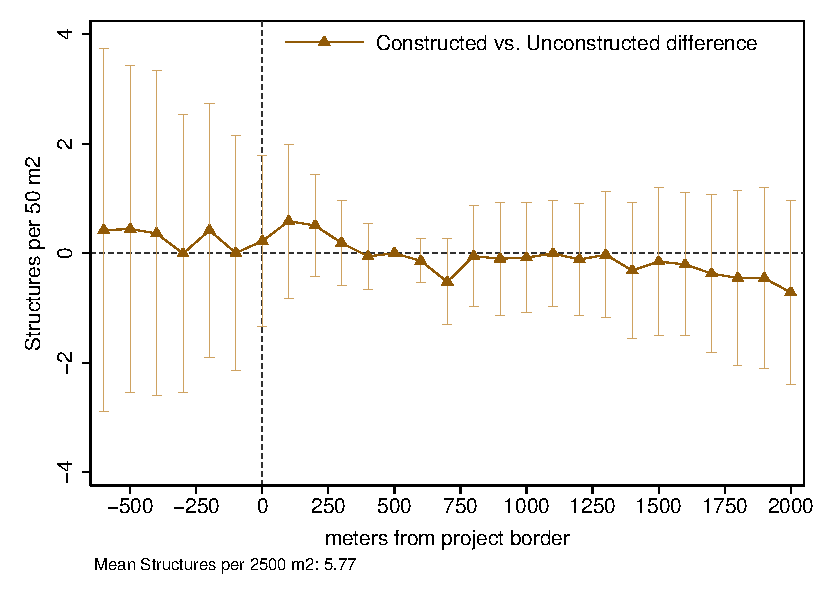
\includegraphics[width=\textwidth,trim={0cm .8cm 0cm .5cm}]{figures/distplotDDD_bblu_total_buildings_admin}
            \caption[Network2]%
            {}    
            \label{fig:prefor}
        \end{subfigure}
        \hfill
        \begin{subfigure}[b]{0.49\textwidth}  
            \centering 
            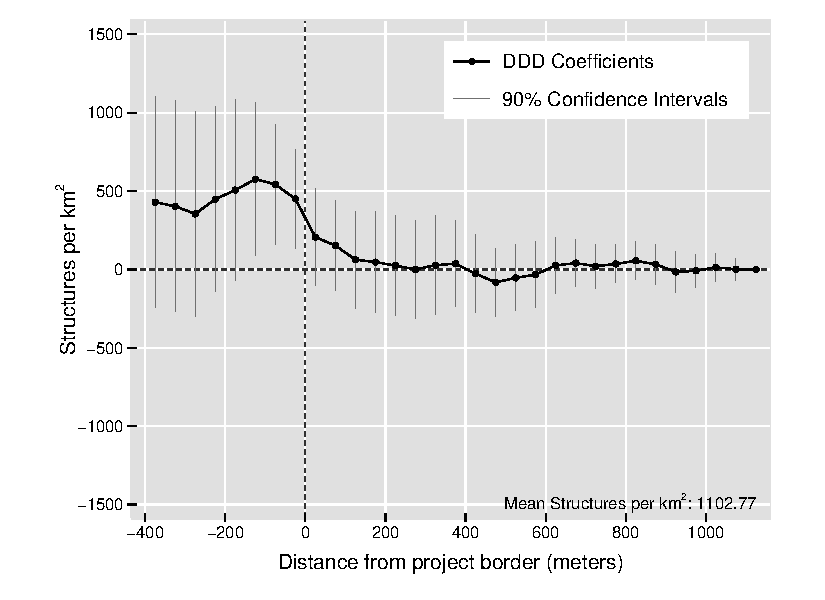
\includegraphics[width=\textwidth,trim={0cm .8cm 0cm .5cm}]{figures/distplotDDD_bblu_for_admin}
            \caption[]%
            {}    
            \label{fig:preinf}
        \end{subfigure}
        \vskip 3mm \vskip 0pt
        \begin{subfigure}[b]{0.49\textwidth}
            \centering
            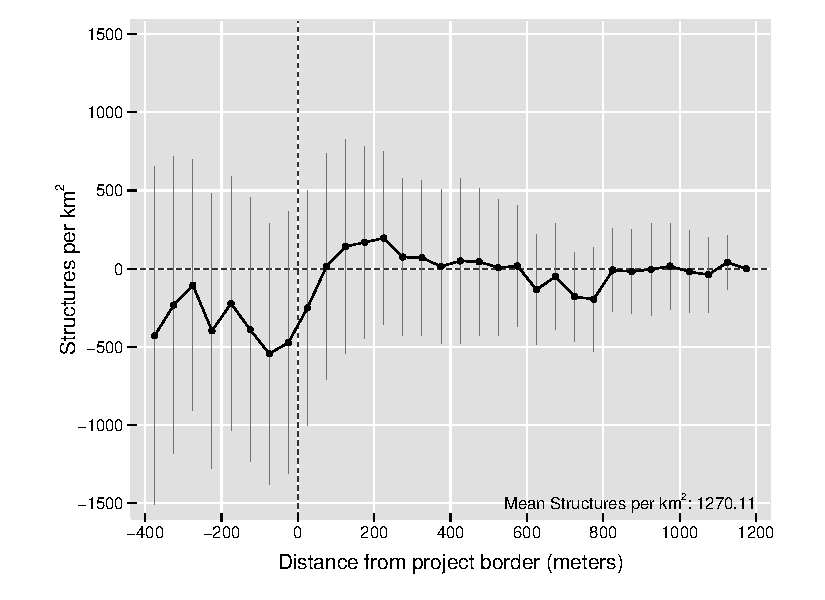
\includegraphics[width=\textwidth,trim={0cm .8cm 0cm .5cm}]{figures/distplotDDD_bblu_inf_admin.pdf}
            \caption[Network2]%
            {}    
            \label{fig:prefor}
        \end{subfigure}
        \hfill
        \begin{subfigure}[b]{0.49\textwidth}  
            \centering 
            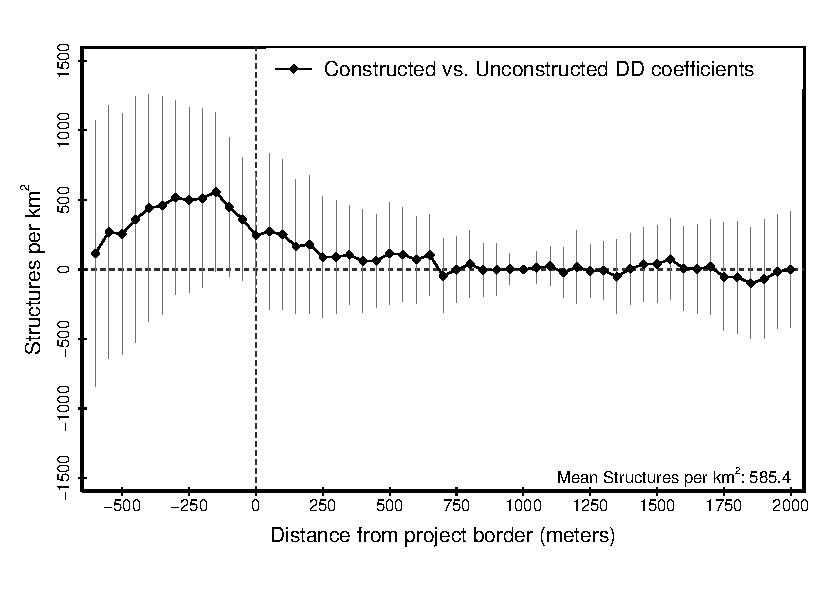
\includegraphics[width=\textwidth,trim={0cm .8cm 0cm .5cm}]{figures/distplotDDD_bblu_inf_backyard_admin}
            \caption[]%
            {}    
            \label{fig:preinf}
        \end{subfigure}
        \vskip -5mm \vskip 0pt
        \begin{subfigure}[b]{0.49\textwidth}  
            \centering 
            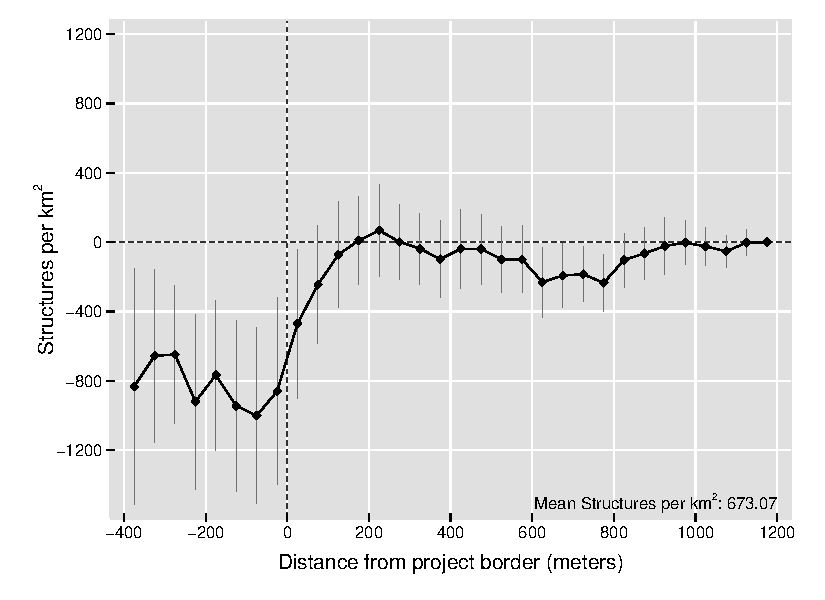
\includegraphics[width=\textwidth,trim={0cm .8cm 0cm .5cm}]{figures/distplotDDD_bblu_inf_non_backyard_admin}
            \caption[]%
            {}    
            \label{fig:preinf}
        \end{subfigure}
        \hfill\quad
        \begin{minipage}[b][6.5cm][c]{0.4\textwidth}   
        \caption[ Housing Densities in Constructed and Unconstructed Projects Areas ]
        {\small Difference-in-differences coefficients for five density outcomes: (a) total housing, (b) formal housing, (c) informal housing, (d) backyard informal housing and (e) non-backyard informal housing.  } 
		\end{minipage}
		\hfill
        \label{fig:rawbblumeans}
    \end{figure*} 

The high geographic resolution of our housing density measure allows us to take a more non-parametric approach to estimating the impacts of housing projects on local building density.  This geographic resolution is instrumental in detecting possible spillover effects just outside of housing project boundaries.  Figure~\ref{figure:housecensusexample} in Appendix~\ref{appendix:bblupictures} demonstrates this resolution by depicting all structures within and around an example housing project.  To construct a measure of housing density, we take the average number of houses within a 50 meter by 50 meter grid cell.  Figure~\ref{figure:housedensityexample} in Appendix~\ref{appendix:bblupictures} provides an example of this density measure over a housing project.  Using these measures, we estimate the following equation:
\begin{equation}
\label{equation:bblu}
y_{ipt} \, = \, \lambda_i + \sum\limits_{d} I^d_{ipt}\Big( \alpha^d D_tC_p \, + \, \beta^dD_t\Big) \, + \, \varepsilon_{ipt}
\end{equation}
$y_{itdp}$ measures the average number of houses for cell $i$ in vicinity of project $p$ observed in year $t$.  We consider four housing density measures: 1) total buildings, 2) formal buildings, 3) informal buildings, and 4) informal backyard shacks.  In this specification, we compute the differential change in density at a variety of distances from project boundaries.  $I^d_{ip}$\,=1 if cell $i$ is at distance $d$ of project $p$.  $D_{t}\,\,$=1 if year $t$ is 2011 again referencing the post period.  $C_{p}\,\,$=1 if project $p$ has been constructed.  In this specification, $\lambda_i$ is a grid-cell level fixed effect.  Interpreting the coefficients of interest, $\alpha^d$, as causal effects of project construction requires a parallel trends assumption at each distance from the project boundary.  

In this context, we are able to perform a more non-parametric comparison of outcomes at baseline.  Figure~\ref{figure:formalmeans} plots simple means of formal housing density with respect to the housing project boundaries (where negative distances track housing density within the boundaries).  Comparing averages for 2001 (black circles), between constructed (left panel) and unconstructed projects (right panel), we find slightly greater formal housing within unconstructed project borders, but nearly identical levels at all distances growing further from boundaries.  Moreover, there does not appear to be a strong gradient in formal housing density moving away from project boundaries.  This flat gradient suggests that while project areas themselves have less development, proximity to these projects is relatively uncorrelated with development.  Therefore, areas further away from projects may additionally serve as plausible comparison groups for areas just outside of housing projects, which may be more likely to experience spillover effects from these projects.



Figure~\ref{figure:formalmeans} also previews the empirical analysis by plotting average formal density for 2011 (orange triangles).  For all positive distances in both panels, we observe a parallel upward shift in formal building density, which does not appear to be correlated with proximity to the project border.  Within the project area (at negative distances), formal housing density increases more substantially for constructed projects than unconstructed projects, consistent with successful project construction.

Figure~\ref{figure:informalmeans} exhibits similar patterns for informal housing density.  Within project areas at baseline (2001), we observe similar average levels of informal housing densities although they are more unevenly distributed for unconstructed projects.  Again, there appears to be little gradient in housing density moving further away from both types of projects.

After construction (in 2011), informal housing density increases across the board although increases are smaller within project areas for constructed projects.  By contrast, informal housing spikes substantially just within unconstructed projects.  Outside of project areas, both types of projects experience parallel shifts in informal housing density that appear uncorrelated with distance from projects.

Taken together, these descriptive results broadly exhibit balance on observable housing densities at baseline.  To the extent that baseline levels in housing density may be correlated with future changes in density, these results provide some additional support for our parallel trends assumptions.


We then estimate equation (\ref{equation:bblu}) to examine the differential changes in housing density between unconstructed and constructed projects.  We present the non-parametric results for formal houses in Figure~\ref{figure:dddformal}, informal houses in Figure~\ref{figure:dddinformal}, and aggregating to total houses in Figure~\ref{figure:dddtotal}.  These figures plot difference-in-differences coefficients for each distance threshold relative to housing project boundaries.  Standard errors are clustered at the project-level for the 57constructed and 60unconstructed areas.  Estimates are especially noisy within project areas because the varying sizes of project footprints mean that observations per distance threshold decline quickly moving further within the footprints.

Figure~\ref{figure:dddformal} finds a substantial increase in formal houses within the project boundary which abruptly shifts to zero moving outside of these projects.  Estimates suggest an housing projects generate increase of 1 formal house per 2500 m2 which is equivalent to around 400 houses per km2, roughly in line with average project density in Table~\ref{table:projectdescriptives}.  These results indicate zero spillovers in terms of formal developments close to these projects, suggesting that these housing projects have minimal local amenity effects.  Figure~\ref{figure:dddinformal} provides the opposite pattern for informal housing with a decrease in density within constructed relative to unconstructed projects.  Positive distances from project areas exhibit zero change in informal housing development indicating a similar lack of spillover effects to neighboring housing stock.  

Taken together, these results suggest that formal project houses crowd-out growth in informal housing leading to zero total change in houses within project areas as demonstrated by Figure~\ref{figure:dddtotal}.  Repeating this exercise for a subset of informal houses coded as backyard shacks, Figure~\ref{figure:dddbackyard} in Appendix~\ref{appendix:backyard} provides additional evidence that stand-alone informal houses are replaced by backyard shacks in constructed project areas.  These results match both the improvements in housing quality as well as the little change in population density detected in the previous census results in Table~\ref{table:censusestimates}.


\section{Price Effects}\label{section:resultsprices}

To identify the spillover effects of public housing on residential home prices in the formal market, we use a similar difference-in-differences approach comparing prices for areas close and far from project areas before and after project implementation.  Our main empirical strategy takes the following specification:

\begin{equation*}
P_{itp} \, = \, \alpha D_{tp}T_{ip} \, + \,\theta_1 D_{tp} \, + \, \,\theta_2 T_{ip}+ \, +  \lambda_p \,  + \, \eta_{t} \, + \, \varepsilon_{itp}
\end{equation*}
% \begin{equation*}
% P_{itp} \, = \, \alpha D_{tp}T_{ip} \, + \,\theta_1 D_{tp} \, + \, \,\theta_2 T_{ip}+ \, X^{'}_{i}\beta \, +  \lambda_p \,  + \, \eta_{t} \, + \, \varepsilon_{itp}
% \end{equation*}
% $X_i$ controls for a quadratic in lot size, which may affect prices over time. 
The outcome, $P_{itp}$, is measured in terms of the log-purchase price of property $i$ sold at time $t$ in the vicinity of project $p$.  To capture changes in prices over time within project areas, $D_{tp}$ is equal to one if date $t$ is after the month of project implementation and zero otherwise.  $T_{ip}$ takes a value of one if property $i$ is within 700m of the project boundary (zero otherwise).  The coefficient of interest, $\alpha$ captures the differential change in prices between near and far properties before and after project construction.   Additionally, $\lambda_p$ includes a project fixed affect controlling for any fixed, unobserved drivers of house prices that vary between projects.  Likewise, $\eta_{t}$ controls for calendar month (year$\,\times\,$month) fixed-effects to account for any factors such as shifts in aggregate housing demand that may be correlated with prices and the timing of housing projects.

Interpreting the coefficient, $\alpha$, as the causal effect of housing projects on nearby home prices requires the following difference-in-differences assumption:
\begin{equation*}
E[\varepsilon_{itp}|X_{i},T_{ip},D_{tp},\lambda_p,\eta_{t}]=0
\end{equation*}
This assumption implies that there are no other factors occurring in the same time and place as the housing projects which may otherwise impact home prices.  One possibility is that housing markets anticipate the construction of these projects so that transactions in the pre-period may be partially treated by the advent of a housing project.  Anecdotal evidence suggests that completion dates for these projects are very uncertain due to the large coordination of stakeholders needed for each project, making it difficult to accurately anticipate implementation.  Another concern would be that housing projects are accompanied by other social programs that would stimulate investments in neighborhoods near project areas.  In order to isolate market anticipation or accompanying social programs from the actual impacts of housing projects, we estimate an identical model for planned but unconstructed projects to test the robustness of the results.  Similarly, in targeting housing projects to particular areas, governments may be responding to local trends in housing markets or economic conditions.  

To separate project impacts from secular market trends, we leverage the sudden roll-out of housing projects under the assumption that market trends are relatively smooth over space and time relative to the construction of housing projects.  In order to non-parametrically assess identification in this way, we also estimate a more flexible model both in terms of distance to project, $D_{tp}$ and time relative to project construction, $T_{ip}$.  Specifically, we estimate separate treatment effects for each 250 meters of distance, $\sum_{d=1}^{8} \alpha_d D_{tpd} T_{ip}$ up to 2000 meters away from the project boundary.  We do not estimate price effects within project boundaries both because (1) there are very few formal transfers of deeds within project boundaries and (2) there is a greater risk of miscoding housing project transactions as outcome transaction within project areas (although we address this mismeasurement below).  We also allow effects to vary according to 12 month intervals relative to construction from three years before and three years after the expected construction date, $\sum_{l=-3}^{3} \alpha_l D_{tp}T_{ipl}$.  All regressions cluster standard errors at the project level in order to account for potential correlation in prices due to unobserved factors within very localized housing markets.  

One concern is that our ability to distinguish between deeds pertaining to project houses and deeds associated with normal house transactions may be imperfect.  Without addressing this concern, we would mistakenly include project house transfers in our outcome measure of normal house transactions, which would substantially bias price effects.  To account for this possibility, we limit our sample to include only seller-names that appear less than 30 times in the data, excluding         28\unskip\% of transactions.\footnote{Results are robust to different thresholds.}  Alongside government housing projects, this approach also mainly excludes large housing developers.  Therefore, the results take a more narrow interpretation as the effect of housing projects on prices for small-scale property owners.  Removing these observations leaves a total sample of     87,253deeds transactions within 2000 meters of a project boundary.

Figure~\ref{figure:distplot} separately plots coefficients for average home prices before construction, $\alpha_{d,pre}$ and after construction, $\alpha_{d,post}$ for each 250m distance ring from housing project boundaries.  The reference category is unconstructed projects 2000m from the project boundary.  The left panel presents price gradients for constructed projects.  For constructed projects, the pre-project gradient slopes slightly upwards consistent with housing projects being located in undeveloped land or preexisting informal settlements, which may have negative amenity effects.  After implementation, the price gradient slopes downwards slightly within 700 meters of the project area suggesting that either housing projects provide a negative amenity value or serve as a local housing supply shock.  The large standard errors on all estimates imply that almost all estimates are no statistically different from zero or each other.

Unconstructed projects in the right panel of Figure~\ref{figure:distplot} exhibit a similarly increasing price gradient before project implementation, again consistent with project land having a negative amenity effect on nearby prices. This gradient remains unchanged in periods after the expected construction date.  These results provide suggestive evidence that the exact location of housing project selection does not appear to be strongly correlated with local housing market trends.
\begin{figure}
\caption{Price Estimates over Distance from Project}\label{figure:distplot}
\centering
Constructed Projects \hspace{3.6cm} Unconstructed Projects
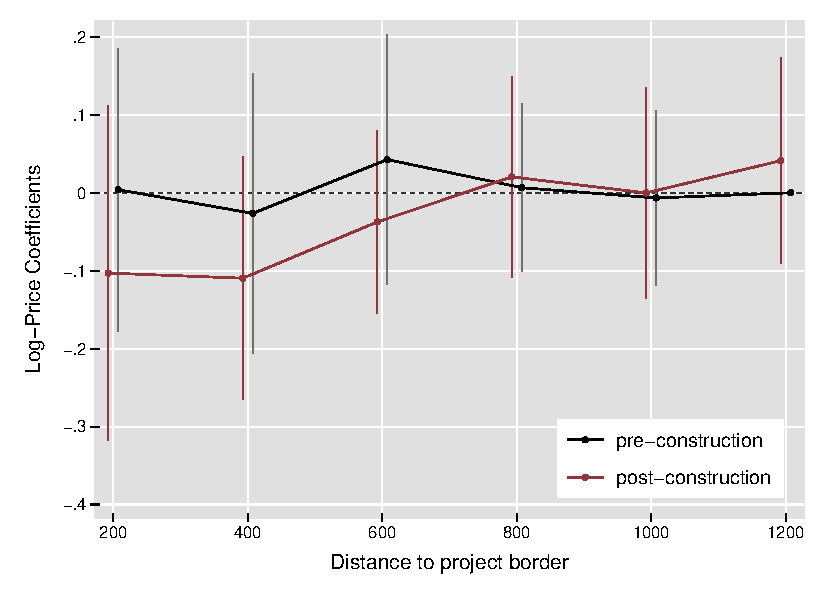
\includegraphics[width=0.44\textwidth,trim={.77cm 0cm .21cm 0cm}]{figures/distance_plot_rdp.pdf}
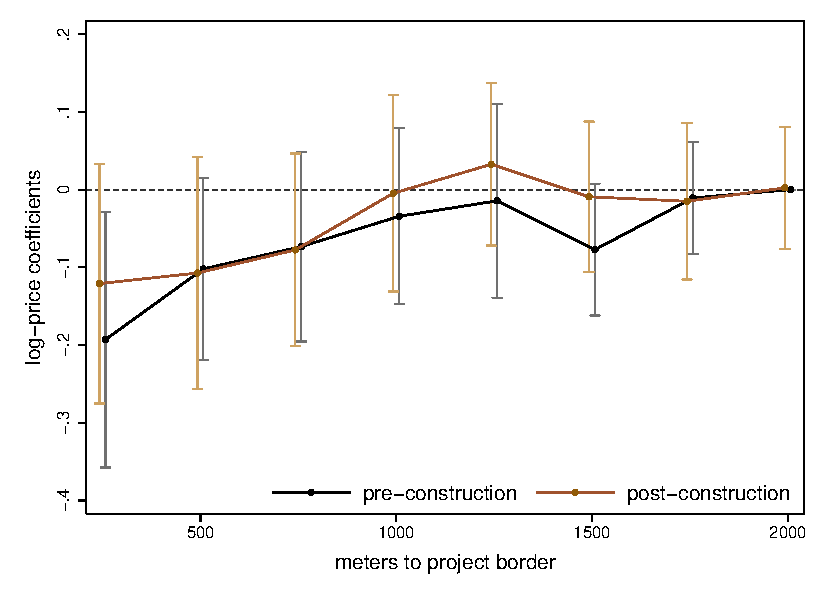
\includegraphics[width=0.44\textwidth,trim={.77cm 0cm .21cm 0cm},clip]{figures/distance_plot_placebo.pdf}\\
\end{figure}
The change in price gradients following project construction (left panel of Figure~\ref{figure:distplot}) is observed to be greatest at distances less than 700 meters from the project boundary.  Given this result, we then use this threshold to define distance rings of ``near'' and ``far'' to examine how prices might change over time relative to date of project construction.

Figure~\ref{figure:timeplot} plots coefficients for average price changes over time relative to the modal construction month for properties within and beyond 700m of a project boundary.  The reference group for this regression is properties further than 700m from a project border in the year before the expected construction date.  

Focusing on constructed projects in the left panel, areas far from project boundaries follow a stable zero trend with respect to the completion of projects.  Meanwhile, areas close to the project boundaries experience a slight but stable decline in prices over the period.  According to the point estimates, the decline is economically significant reaching 15\% below average prices (given that the outcome is log-prices).  This decline may provide evidence of anticipatory behavior: local homeowners hear news about a new housing project and decide to sell their houses, anticipating a price drop due to the housing project.

For unconstructed projects in the right panel, areas far and near from project boundaries follow similar parallel trends to constructed projects leading up to the expected completion date and remain indistinguishable for the entire duration after this date.  This null result helps to exclude competing explanations that rely on the timing of housing projects such as targeting housing programs according to hyper-local housing market trends or pairing housing projects with other place-based policies.  One caveat for these results is that measurement error both in matching project names to budget statements and in assigning the proper date of completion for each project may bias results toward zero.  It is unclear the extent to which anticipation effects might have a role in this case; if nearby homeowners have little information on when a project will be constructed, then we should expect to see the same anticipation effects as for constructed projects.  However, if local homeowners are well informed about the local dynamics determining project construction, then anticipation effects would likely be more muted in the case of unconstructed projects.
\begin{figure}
\caption{Price Estimates over Time}\label{figure:timeplot}
\centering
Constructed Projects \hspace{3.6cm} Unconstructed Projects
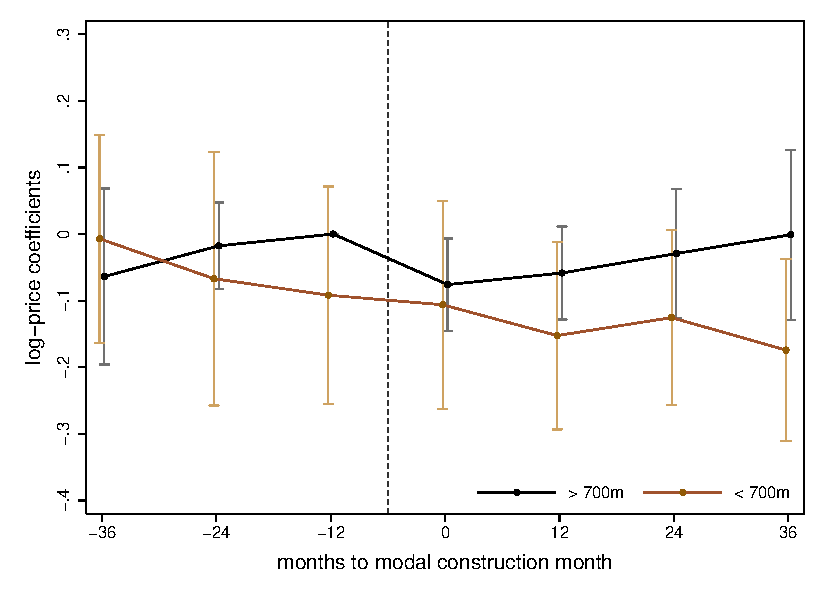
\includegraphics[width=0.44\textwidth,trim={.77cm 0cm .21cm 0cm}]{figures/time_plot_rdp.pdf}
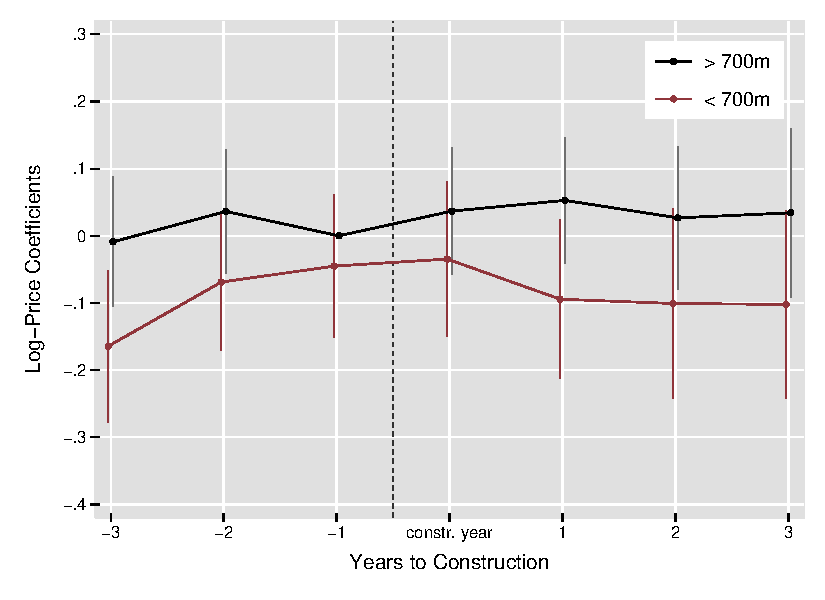
\includegraphics[width=0.44\textwidth,trim={.77cm 0cm .21cm 0cm},clip]{figures/time_plot_placebo.pdf}
\end{figure}
To test the significance of these effects in a regression framework, we first run two simple difference-in-differences regressions separately for constructed and unconstructed projects where ``Post'' is defined as anytime after expected project construction and ``Near'' includes properties within 700m of project boundaries.  We also conduct a triple-differences analysis which adds the indicator $C_{it}$ for whether a project is constructed as well as the full set of interaction terms with this indicator in the following equation:
\begin{equation*}
P_{itp} \, = \, \alpha D_{tp}T_{ip} C_{it} \, + \,\theta_1 D_{tp} \, + \, \theta_2 T_{ip}+ \, \theta_3 C_{it}+ \, \theta_4 D_{tp} T_{ip} \, + \, \theta_5 C_{it} T_{ip}  \, + \, \theta_6 C_{it} T_{ip} \, +  \lambda_p \,  + \, \eta_{t} \, + \, \varepsilon_{itp}
\end{equation*}
This triple-differences specification allows for a slightly less restrictive form of parallel trends: instead of requiring price changes to be parallel close and far from a project, this approach simply requires that differential price changes close and far from a project for constructed areas would be the same in unconstructed project areas in the absence of construction.  

Table~\ref{table:priceest} provides the estimation results with results for constructed projects in the first column, unconstructed projects in the second column, and finally triple-difference estimates in the third column.  The coefficient of interest in the first column, $Post X Near$, translates the declining price gradient for nearby properties in constructed project areas in Figure~\ref{figure:timeplot} to a 7.5\% decrease in house prices which is significant at the 10\% level.  The corresponding difference-in-differences coefficient for planned but unconstructed projects in the second column predicts a much smaller and statistically insignificant decline in prices.  Pooling samples in the third column, the triple-difference coefficient of interest captures roughly the midpoint between the constructed and unconstructed difference-in-differences coefficients, resulting in a noisy 6\% decline in house prices.  Meanwhile to put this effect into perspective, being within 700m or in a constructed area both shift mean prices by 12\%, which are statistically significant at the 5\% level.  Taken together, these results provide weak evidence of a slight decline in home prices, which seem to be more driven by anticipation of project completion than by the direct impact of nearby formal housing.
\begin{table}
\caption{Price Estimates for Completed Projects}\label{table:priceest}
\centering
\begin{tabular}{lccc} \hline
 & (1) & (2) & (3) \\
VARIABLES & Const & Unconst & All \\ \hline
 &  &  &  \\
Post X Near X Const. &  &  & -0.0597 \\
 &  &  & (0.0665) \\
Post X Const. &  &  & 0.00354 \\
 &  &  & (0.0469) \\
Near X Const. &  &  & 0.0662 \\
 &  &  & (0.0676) \\
Post X Near & -0.0747* & -0.0325 & -0.0253 \\
 & (0.0414) & (0.0413) & (0.0495) \\
Post & 0.0332 & 0.0407* & 0.0277 \\
 & (0.0219) & (0.0239) & (0.0306) \\
Near & -0.0280 & -0.151*** & -0.126** \\
 & (0.0421) & (0.0453) & (0.0546) \\
Const. &  &  & -0.129** \\
 &  &  & (0.0543) \\
Constant & 10.36*** & 7.868*** & 10.59*** \\
 & (0.265) & (0.310) & (0.237) \\
 &  &  &  \\
Observations & 41,881 & 34,146 & 87,253 \\
R-squared & 0.348 & 0.348 & 0.330 \\
Year-Month FE & Yes & Yes & Yes \\
 Project FE & Yes & Yes & Yes \\ \hline
\multicolumn{4}{c}{ Robust standard errors in parentheses} \\
\multicolumn{4}{c}{ *** p$<$0.01, ** p$<$0.05, * p$<$0.1} \\
\multicolumn{4}{c}{ Clustered at the project level.} \\
\end{tabular}
 \\
\footnotesize{Outcomes are in log-purchase prices. ``Const'' refers to constructed while \\ ``Unconst'' refers to unconstructed housing projects.}
\end{table}


\section{Discussion and Conclusion}\label{section:discussion}

We find that South African housing projects greatly improve the housing conditions within their footprints.  Housing projects successfully deliver large numbers of new formal structures (Figure~\ref{figure:dddformal}) and much better access to bulk services (Table~\ref{table:censusestimates}).  At the same time, formal project housing appears to crowd-out growth in informal settlements so that the total density of housing remains the same as in unconstructed project areas (Figure~\ref{figure:dddtotal}).  Moreover, results in Table~\ref{table:censusestimates} indicate that the average quality of new project houses are at least as good as neighboring houses at baseline.  Therefore consistent with the model of amenity effects in \cite{diamond2016wants}, we would expect to find that these programs increase nearby home prices; however, results in Table~\ref{table:priceest} report if anything the opposite trend.  Similarly, we do not observe large new developments in either informal or formal housing just nearby these projects.

The lack of significant spillover effects in price as well as in quantity is consistent with countervailing amenity and housing supply effects.  While an influx of new houses threatens to decrease prices and housing supply nearby, positive amenities provided by housing projects may also attract greater housing investment, increasing prices.  While both amenity and supply effects predict increases in local population, there may be spatial or geographic constraints on population growth given that these settlements in South Africa are almost exclusively single-story and informal settlements often fill any remaining surface area.

Our interpretation is encouraging from a policy perspective: housing projects can produce enough positive amenities to mediate any housing supply effects.  Additionally, these projects effectively replace informal settlements with high quality formal houses, achieving a signature goal of South Africa's policy.  At the same time, there is little evidence supporting housing policy as an important engine for local economic growth and development.  These results may at least mediate any concerns policymakers may have for adversely affecting communities with housing projects, despite sometimes loud complaints from nearby community members.

It is important to emphasize that our analysis does not currently speak to the overall welfare implications of these policies.  For example, public housing may lead to an overall net reduction in slums in the city, which may generate total welfare gains through fewer congestion externalities or other mechanisms.  In light of South Africa's emphasis on using housing policy to stimulate neighborhood development, we hope that this paper will be useful for policymakers in considering the range of informal housing market responses as they design new housing policies.

%\section{Conclusion}\label{section:conclusion}
%This paper serves as a cautionary tale for low-density public housing in developing countries.  While these projects may be designed to improve local housing markets and reduce local slum growth, they may instead support local slum growth through a mix of available land and improved infrastructure.  It is important to emphasize that our analysis does not currently speak to the overall welfare implications of these policies.  For example, public housing may lead to an overall net reduction in slums in the city, which may generate total welfare gains through fewer congestion externalities or other mechanisms.  According to our model, the optimal housing policy depends crucially on the shape of these congestion externalities.  We look forward to using variation in the South African housing program to estimate these externalities in future work.  





\pagebreak
\nocite{*}
\singlespacing
\setlength{\bibsep}{7pt}
\bibliographystyle{abbrvnat}
\bibliography{ref}



\pagebreak
% APPENDIX 
\appendix
\doublespacing

\section{Appendix}

\subsection{String Matching for Project Names}

\begin{table}
	\centering
	\caption{Assessing Name Matching between \\Budget and Spatial Administrative Data}\label{table:stringmatch}
\begin{tabu}{lcc}
 & Matched  & Unmatched  \\
\midrule
 Formal Density: 2001  & 230.5  & 171.5  \\ 
 Formal Density: 2011  & 814.1  & 444.0  \\ 
 &  &  \\ 
 Informal Density: 2001  & 1,055.6  & 1,401.0  \\ 
 Informal Density: 2011  & 1,613.2  & 2,147.0  \\ 
 &  &  \\ 
 Project House Density  & 125.0  & 66.0  \\ 
 Project Mode Year  & 2005  & 2005  \\ 
 &  &  \\ 
 Hectares  & 97.3  & 119.6  \\ 
 &  &  \\ 
\midrule
 Observations  & 322  & 320  \\ 
\bottomrule
\end{tabu}
 \\
Density is measured in structures per $\text{km}^{2}$.

\end{table}


\subsection{Census Block Analysis}

\begin{figure}
\caption{Buffer Design Census Block Example}\label{figure:bufferdesigncensus}
\centering
\tcbox[colback=white,boxrule=.35mm,boxsep=0mm]{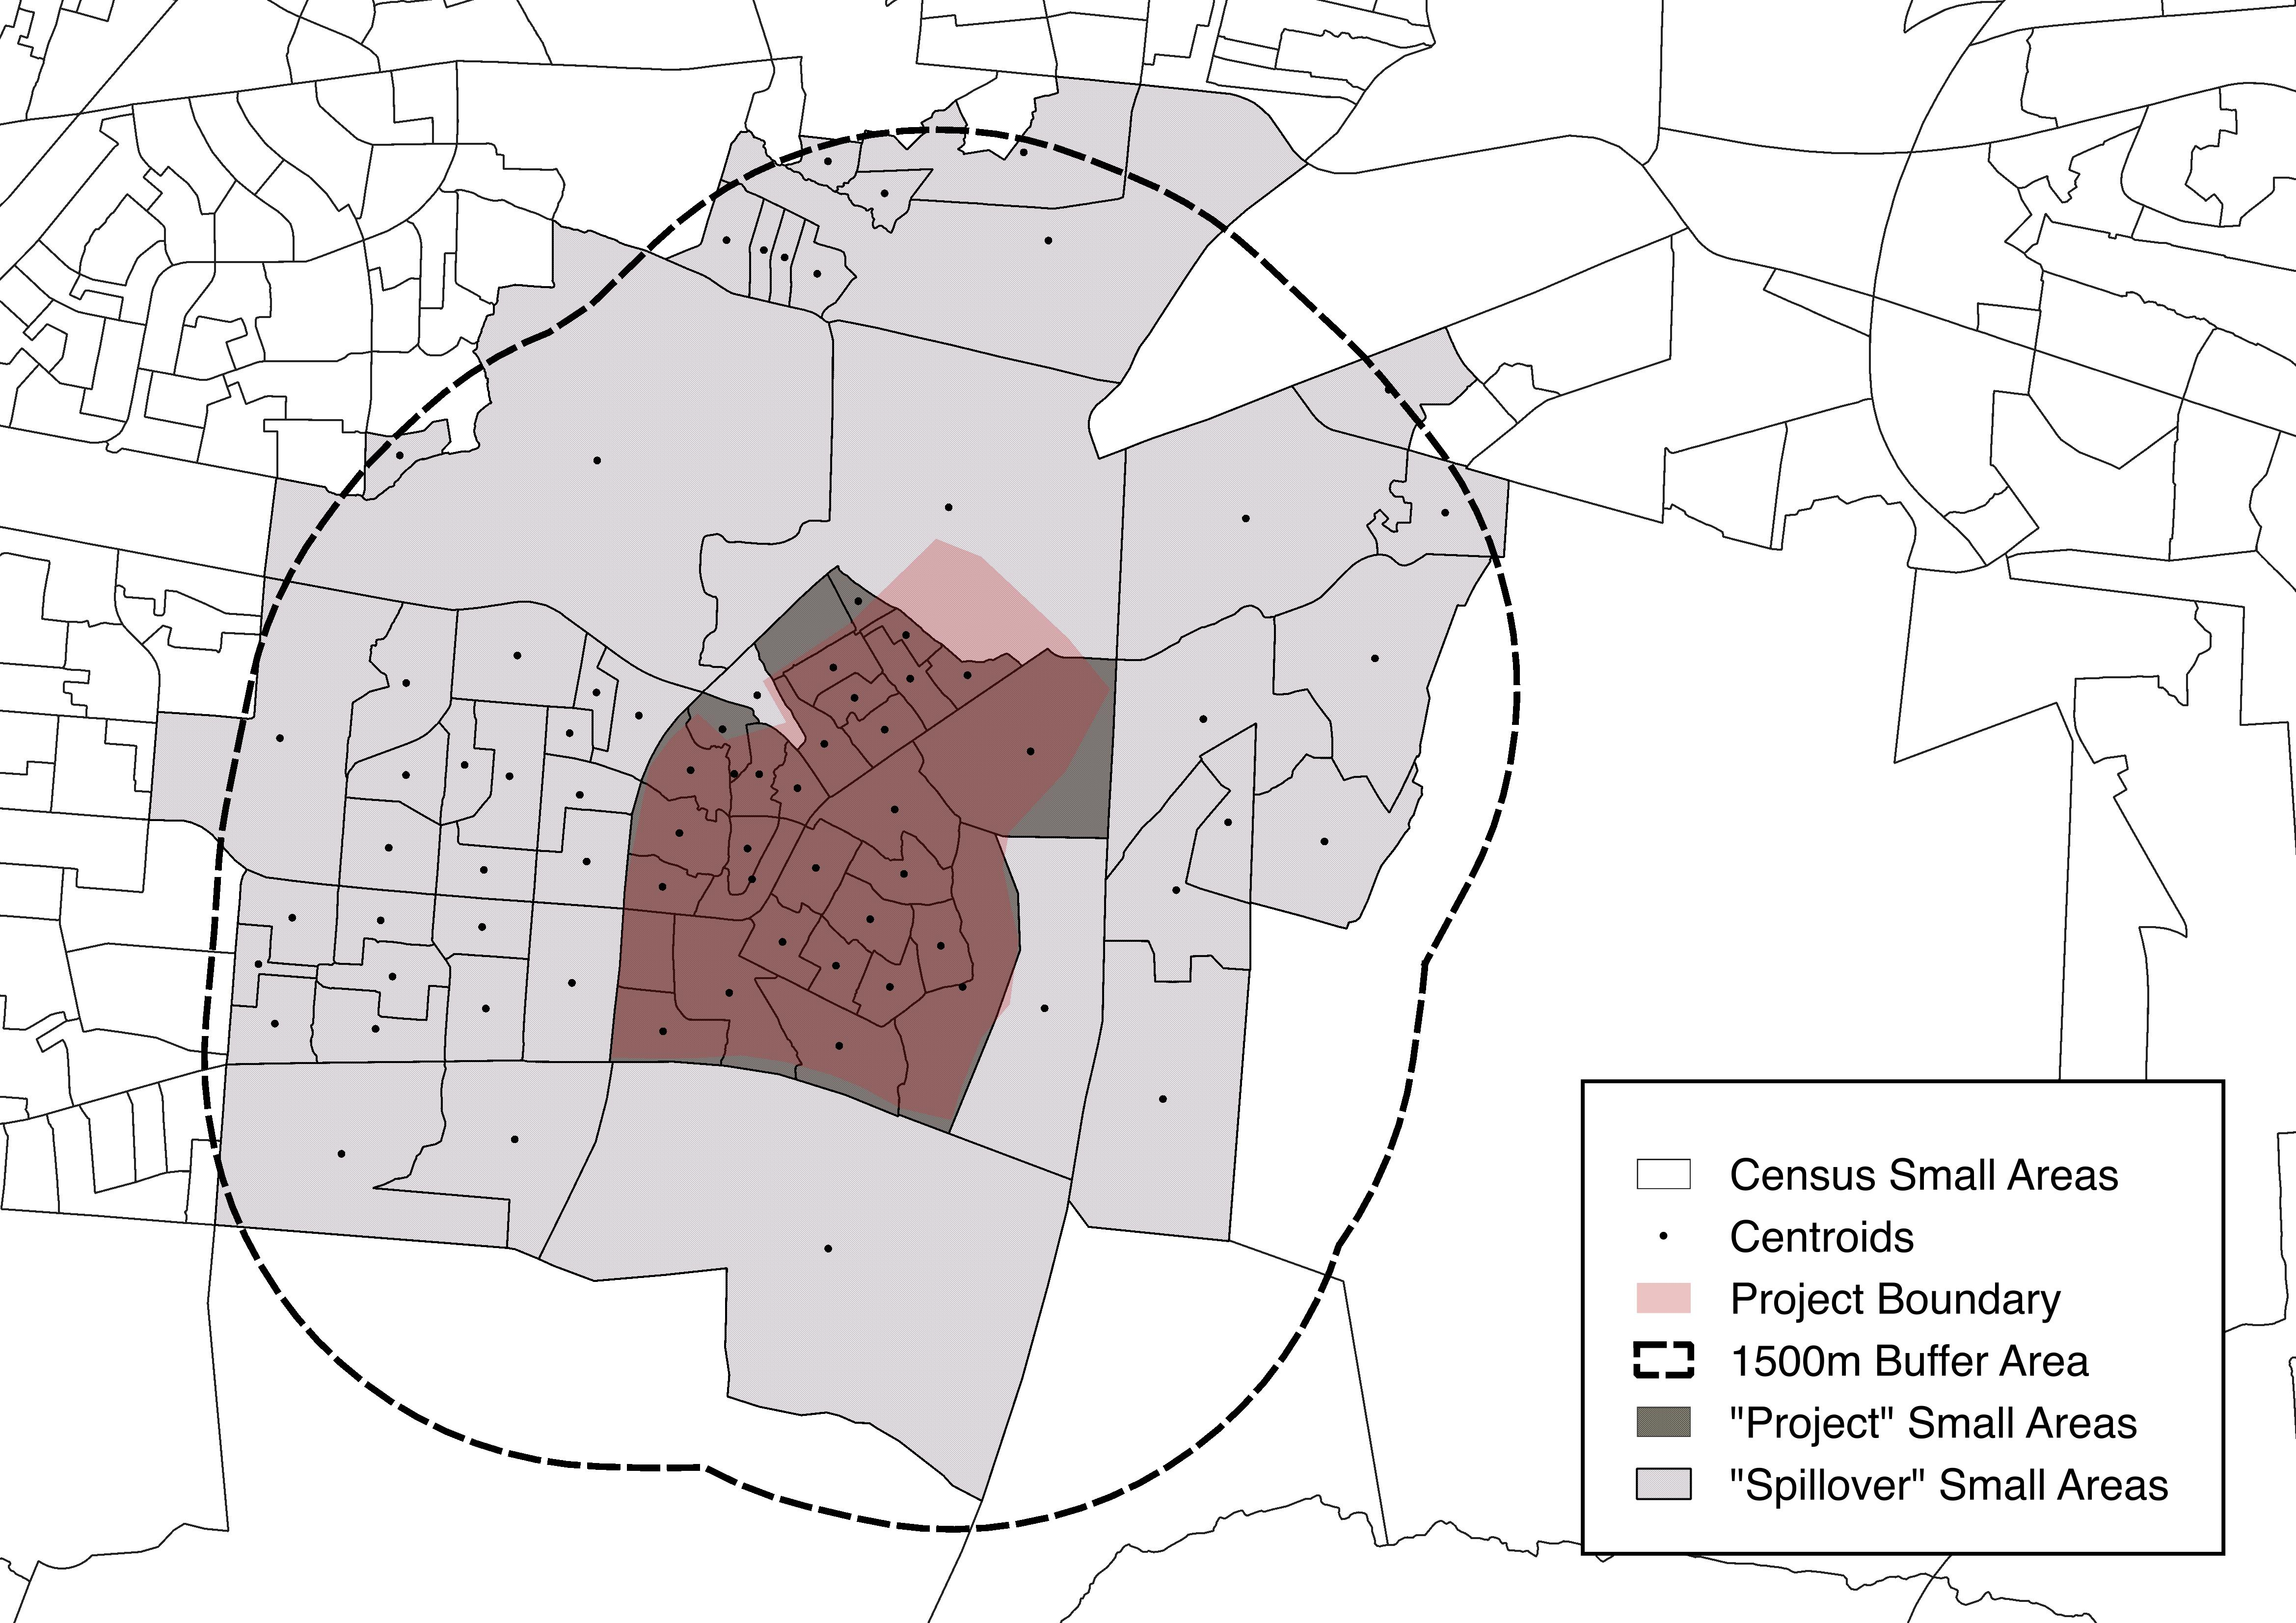
\includegraphics[scale=.47,trim={.75cm .4cm .75cm .4cm}]{figures/census_design.jpg}} 
\end{figure}




\end{document}



%%%%%% OLD BUILDING GROWTH AROUND HOUSING PROJECTS 

% \subsection{Building Growth around Housing Projects}


% Using the building survey, we provide a first look at housing development around completed and uncompleted projects.  Figure~\ref{figure:buildingchanges} plots the average number of new structures between 2001 and 2011 in distance rings from the boundary of both completed and uncompleted project areas.  Negative distances measure new structures within the project areas themselves.  

% Focusing on completed projects in the left panel, strong growth in formal residential structures at negative distances provides another measure of the direct impact of the housing projects.  We also observe strong growth in informal residential structures within project areas.  This finding is consistent with anecdotal evidence from fieldwork in South Africa pointing to the prevalence of backyard shacks where owners of project houses use their land plots to construct informal housing.  At positive distances, the growth in formal structures immediately dissipates while the growth in informal structures remains substantial up to at least 400 meters from the project border.  This sustained growth in nearby informal dwellings matches a common complaint of local housing authorities and NGOs who notice crowding-in of slum areas around project areas in order to utilize the public services offered within the projects.  	

% Results for uncompleted projects in the right panel indicate a similar pattern of informal structure growth in project areas.  However compared to completed projects, lower levels of formal structure growth occur within uncompleted project footprints before quickly dissipating outside of the projects.  Informal structure growth also decreases suddenly outside of the projects.  This result suggests that completed housing projects may play an important role in generating nearby growth in informal settlements in the right panel.  The flat, smooth trends in structure growth past 500 meters for both completed and uncompleted projects support interpreting these regions as capturing the types of local development that we might expect in the absence of the housing projects.




%%%%%%%%%%%%%%% HERE IS THE OLD CENSUS ANALYSIS %%%%%%%%%

% To provide additional evidence on how the demographics and infrastructure may be changing as a result of these projects, we use a slightly modified differences-in-differences design where uncompleted project areas are directly treated as counterfactuals.  The specification for analyzing the census data takes the following form:
% \begin{equation*}
% Y_{hbtp} \, = \, \alpha_{O} D_{tp} T_{bp} O_{bp} \, + \alpha_{S} D_{tp} T_{bp} S_{bp} \, + \,\theta_1 D_{tp} O_{bp} + \,\theta_2 D_{tp} S_{bp} \, + \theta_3 T_{bp} S_{bp}  \, +  \, \theta_4 S_{bp} \, +  \lambda_p \, + \, \varepsilon_{hbtp}
% \end{equation*}
% The outcome, $Y_{btph}$, includes demographic characteristics for household (or person) $h$ living in census block $b$ and project area $p$ in year $t$.  $O_{bp}$ takes a value of one for census blocks with greater than 30\% area overlap with housing projects (zero otherwise) while $S_{bp}$ is the converse identifying ``spillover'' census bocks that have less than 30\% overlap but whose centroids are still within a 1.2 km buffer of the housing project boundaries.  To account for secular changes in outcomes between 2001 and 2011 affecting all census blocks, $D_{tp}$ is equal to one if year $t$ is equal to 2011 and zero otherwise.  $T_{ip}$ takes a value of one for census blocks near completed projects and a value of zero for census blocks near uncompleted projects.  Controlling for differential time trends for overlap and spillover projects, $D_{tp} O_{bp} $ and $D_{tp} S_{bp}$ as well as separate means for both completed, $T_{bp} S_{bp}$, and uncompleted, $S_{bp}$, spillover areas leaves census blocks that overlap with uncompleted projects in the pre-period as the reference group.  $\lambda_p$ includes a project-level fixed effect to control for fixed differences in census characteristics between different projects.  The coefficients of interest, $\alpha_O$ and $\alpha_{S}$, capture differential changes in outcomes between completed and uncompleted projects separately for overlapping and spillover census blocks.  

% To interpret the coefficients, $\alpha_O$ and $\alpha_S$, as the causal effects of housing projects on both overlapping and spillover outcomes, we make the following assumption:
% \begin{equation*}
% E[\varepsilon_{hitp}|T_{ip},D_{bp},S_{bp},O_{bp},\lambda_p]=0
% \end{equation*}
% Intuitively, this assumption requires that there are no other factors occurring at the same time both within and around the completed housing projects that may drive changes in local demographics.  By limiting the control group to only include uncompleted projects, we make the following parallel trends assumption: outcomes near completed projects would have evolved in the same ways as outcomes near uncompleted projects in the absence of the housing projects.  This design leverages similarities in areas around completed and uncompleted projects rather than comparing project areas to the entire region of Gauteng.  To the extent that locations of housing project may be targeted to local economic conditions, other areas in the province may be less likely to satisfy parallel trends assumptions.  

% At the same time, local economic and political conditions may determine which projects are completed and which are either canceled or delayed.  To the extent that these conditions may be correlated with changes in local demographics, the assumption of parallel trends would not hold in the analysis.  Table~\ref{table:censusdescriptives} and Table~\ref{table:projectdescriptives} provide evidence that uncompleted project areas have more informal settlements and fewer services at baseline, consistent with policymakers placing less priority on finishing projects in these areas.  At the same time, spillover areas appear very similar in Table~\ref{table:censusdescriptives} suggesting that differences in trends in these areas may be more plausibly associated with completion of housing projects.  


%%%%% OLD MODEL WRITE-UP !$!$!$!$!$!$!$!$!$!$!$


% We develop a simple model of residential choice in order to both guide the reduced form empirical analysis as well as provide a framework evaluating the welfare effects of public housing policy.  The key insight of the model is that while public housing projects provide high-quality houses and infrastructure, they also cross-subsidize informal housing markets, which can exacerbate congestion externalities and decrease prices in the formal market.

% \subsection*{Basic Setup}
% A city is comprised of $N$ residential neighborhoods indexed $n\in\{1,...,N\}$.  Each neighborhood has a formal and informal housing sector, indexed $s\in\{F,I\}$.  Each neighborhood is distinguished by its local housing supply and later by negative congestion externalities from informal housing.  All jobs are in the central business district and pay a fixed wage rate, and commuting to the CBD is costly.

% \subsection*{Housing Demand}

% Measure one of freely-mobile agents inelastically demand one unit of housing. An agent $i$ has idiosyncratic tastes for neighborhoods, represented by the vector $\bm{\epsilon}_i \in \mathbb{R}^{2N}$ of neighborhood-sector specific valuations. The distribution of preferences in the population is given by the continuous and well-behaved function $f(\bm{\epsilon})$ such that $\int f(\bm{\epsilon}) d\bm{\epsilon} = 1$.
% The indirect utility of individual $i$ living in sector $s$ of neighborhood $n$ is given by:
% \begin{equation*}
% \begin{aligned}
% u_{ins} \,& =\, A_{ns}\,-\, R_{ns} \,+\, \epsilon_{ins} \\
%         \,& =\, v_{ns} \,+\, \epsilon_{ins}
% \end{aligned}
% \end{equation*}
%  where $A_{ns}$ may be interpreted as the net-of-commuting and amenity-adjusted wage received in $n$ when living in sector $s$, $R_{ns}$ is the rental rate of housing, and $\epsilon_{ins}$ is individual $i$'s idiosyncratic taste for neighborhood-sector pair $(n,s)$.  In this framework, neighborhood-sector tastes, $\epsilon_{ins}$, are assumed to be uncorrelated across space and sector.  This assumption rules out cases where households may prefer living closer to certain areas or in certain types of housing.

%  For notational convenience, we denote the array of quantities $A_{ns}$, $R_{ns}$ and $\epsilon_{ins}$ in their matrix form as $\bm{A}$, $\bm{R}$ and $\bm{\epsilon}_i$. Individual $i$ takes exogenous quantities $\{\bm{A},\bm{\epsilon}_i\}$ and endogenous rents $\bm{R}$ as given, and locates in pair $(n,s)$ yielding the highest indirect utility. Aggregate housing demand $H_{ns}$ in $(n,s)$ is given by:
% \begin{equation*}
% \begin{aligned}
% H_{ns} \,\,& =\,\, \int I\Big( \, u_{ins} \,=\, \max_{n's'}\{u_{in' s'} \,\,|\,\, \bm{A},\bm{R}\,\} \Big)f(\bm{\epsilon}) d\bm{\epsilon}    \\[.2em]
%         \,\,& =\,\, D_{ns}(\bm{A},\bm{R})
% \end{aligned}
% \end{equation*}


% \subsection*{Housing Supply}

%  Neighborhoods are endowed with $L_n$ units of land. A share $\theta_{nF}$ of the total land stock is available for formal residential development, while the rest, $\theta_{nI} = 1-\theta_{nF}$, is vacant or public land suited for informal housing. We assume that $\theta_{nF}$ is determined exogenously. In each sector, price-taking landlords supply housing by combining land and materials $M$ with CRS technology $q(L,M)$. Materials are supplied at fixed cost $c$ on a large national market. Because land is fixed in every market, the marginal cost of housing is increasing. The government may also choose to subsidize housing in market $(n,s)$ at a rate of $\delta_{ns}$ per unit. The inverse supply curve in $(n,s)$ is:
% \begin{equation*}
% R_{ns} \,\, =\,\, S(H_{ns},\theta_{ns}L_n) - \delta_{ns}
% \end{equation*} \\[-1.99em]
%  where $\partial S/\partial H > 0$ and $\partial S/\partial L < 0$. For notational convenience, we denote the array of quantities $H_{nh}$, $L_n$ and $\theta_n$ in their vector form as $\bm{H}$, $\bm{L}$ and $\bm{\theta}$, respectively.

% \subsection*{Equilibrium}

% Given density $f(\bm{\epsilon})$ and the exogenous quantities $\{\bm{A},\bm{L},\bm{\theta}\}$, an equilibrium in this city consists of rents $\bm{R}^*$ and housing quantities $\bm{H}^*$ such that all housing markets clear, that is, $\forall (n,h)$:
% \begin{equation}
% \begin{aligned}
% & H^*_{ns} \,\, =\,\, D_{ns}(\bm{A}, \bm{R}^*) \\
% \text{and}\quad & R^*_{ns} \,\, =\,\, S(H^*_{ns},\theta_{ns}L_n) - \delta_{ns} \text{,}
% \end{aligned}
% \end{equation}\\[-1.99em]\\[-1.99em]
%  and all agents live somewhere:
% \begin{equation*}
% \sum_{n}\sum_{s} H^*_{ns} = 1 
% \end{equation*} \\[-1.99em]

% \subsection*{Welfare Implications of Housing Subsidies}

%  The sum of individuals' utility is given by:
% \begin{equation*}
% U \,\, =\,\, \int \max_{n's'}\{u_{in' s'}\,\,|\,\, \bm{A},\bm{R}^*\,\}f(\bm{\epsilon}) d\bm{\epsilon} 
% \end{equation*} \\[-1.99em]
%  and total landlords' profit is:
% \begin{equation*}
% \begin{aligned}
% \Pi \,\, &=\,\, \sum_{n}\sum_{s} \Bigg(\,\int_0^{H^*_{ns}} [R^*_{ns} - (S(x,\theta_{ns}L_n) - \delta_{ns})]dx \, \Bigg) \\[.6em]
% \,\, &=\,\, \sum_{n}\sum_{s} \Bigg(\, R^*_{ns}H^*_{ns} +  \delta_{ns}H^*_{ns} -  \int_0^{H^*_{ns}}S(x,\theta_{ns}L_n)dx  \,\Bigg)
% \end{aligned}
% \end{equation*} \\[-1.99em]
%  Total social welfare in this economy is therefore $W = U + \Pi$. We are interested in the welfare implications of the government subsidizing formal housing in a subset $\mathcal{N}\subset\{1,...,N\}$ of neighborhoods. Let $\delta_{ns}=\delta$ if $n\in\mathcal{N}$ and $s=F$, and $\delta_{ns}=0$ otherwise.  To characterize the marginal social benefit from the subsidy, $\partial W/\partial \delta$,  we first note a result shown in \cite{busso2013assessing}:

% \begin{equation*}
% \begin{aligned}
% \frac{\partial U}{\partial v_{ns}} \,\, & =\,\, \int \frac{\partial }{\partial v_{ns}} \max_{n's'}\{u_{in' s'}\,\,|\,\, \bm{A},\bm{R}\,\}f(\bm{\epsilon}) d\bm{\epsilon} \\[.6em]
% \,\, & =\,\, \int I\Big( \, u_{ins} \,=\, \max_{n's'}\{u_{in' s'} \,\,|\,\, \bm{A},\bm{R}\,\} \Big)f(\bm{\epsilon}) d\bm{\epsilon} \\[.6em]
% \,\, & =\,\  H_{ns}
% \end{aligned}
% \end{equation*} \\[-1.99em]

%  Using the above, we write the derivative of total utility with respect to subsidy $\delta$ as:

% \begin{equation*}
% \frac{\partial U}{\partial\delta} \,\,=\,\,  \sum_{n}\sum_{s}\,\, H^*_{ns}\Big(-\frac{\partial R_{ns}^*}{\partial \delta}\Big) 
% \end{equation*} \\[-1.99em]

%  The derivative of total profits with respect to $\delta$ is:

% \begin{equation*}
% \frac{\partial \Pi}{\partial\delta} \,\,=\,\, \sum_{n\in\mathcal{N}} H^*_{nF} \,\,+\,\, \sum_{n}\sum_{s}\, \Big[ H^*_{ns}\frac{\partial R^*_{ns}}{\partial \delta} \,\,+\,\, R^*_{ns}\frac{\partial H^*_{ns}}{\partial \delta} \,\,+\,\, \delta_{ns}\frac{\partial H^*_{ns}}{\partial \delta} \,\,-\,\, \frac{\partial H^*_{ns}}{\partial \delta}\big( R^*_{ns} \,\, + \,\, \delta_{ns} \big) \Big]
% \end{equation*} \\[-1.99em]

%  Summing and simplifying:

% \begin{equation}
% \frac{\partial W}{\partial\delta} \,\,=\,\, \frac{\partial U}{\partial\delta} \,\,+\,\, \frac{\partial \Pi}{\partial\delta} \,\,=\,\, \sum_{n\in\mathcal{N}} H^*_{nF}
% \end{equation} \\[-1.99em]

%  The total cost of the subsidy is given by $TC = \sum_n\sum_s H^*_{ns}\delta_{ns}$ and its marginal cost is thus:
% \begin{equation*}
%  \frac{\partial TC}{\partial \delta} \,\,=\,\, \sum_{n\in\mathcal{N}} \Big( H^*_{nF} \,\,+\,\, \delta\frac{\partial H^*_{nF}}{\partial \delta} \Big)
%  \end{equation*} \\[-1.99em]

%   The extra term in this expression relative to (2) represents the marginal deadweight loss from an increase in $\delta$. Unsurprisingly, we find that subsidies in an economy with perfect housing markets lead to economic inefficiencies. Furthermore, the magnitude of these inefficiencies depends critically on the population responses in subsidized markets.

%  \subsection*{Housing subsidies with Slum Externalities}

%  Densely populated slums pose fire hazards, increase health risks and overburden existing public infrastructure, e.g. water and sewage networks. We consider an external utility cost from informal housing of the form:

% \begin{equation*}
% A_{ns} \,\,=\,\, \bar{A}_{ns} \,\,+\,\, a\Big(\frac{H_{nI}}{L_n}\Big)
% \end{equation*} \\[-1.99em]

%  where $a'(.)<0$. With this specification, the private decision of locating in $(n,I)$ negatively impacts all residents in $n$ because of congestion effects. The utility response to $\delta$ now depends on how both rents and amenities change in equilibrium:

% \begin{equation*}
% \frac{\partial U}{\partial\delta} \,\,=\,\,  \sum_{n}\sum_{s} \,\, H^*_{ns}\Big(a'\Big(\frac{H^*_{nI}}{L_n}\Big)\frac{\partial H^*_{nI}}{L_n\partial \delta}\,\,-\,\,\frac{\partial R_{ns}^*}{\partial \delta}\Big) 
% \end{equation*} \\[-1.99em]

%  Therefore:

% \begin{equation*}
% \frac{\partial W}{\partial\delta} \,\,=\,\, \sum_{n\in\mathcal{N}} H^*_{nF} \,\,+\,\, \sum_{n} a'\Big(\frac{H^*_{nI}}{L_n}\Big)\,\frac{\partial H^*_{nI}}{\partial \delta}\,\frac{(H^*_{nF}+H^*_{nI})}{L_n}
% \end{equation*} \\[-1.99em]

%  Combining the equilibrium conditions in (1) and using the implicit function theorem, it is possible to show formally that $\partial H^*_{nI}/\partial \delta < 0 \,\,\forall n$. The extra term in the above expression -- relative to equation (2) -- represents the marginal welfare {\it gain} from reduced slum density. The subsidy $\delta$ makes formal housing in $\mathcal{N}$ more attractive relative to informal housing. Marginal residents moving to $\mathcal{N}$ make remaining residents better-off because of reduced congestion. The marginal deadweight loss (MDWL) of the subsidy is now :

% \begin{equation*}
% \begin{aligned}
% MDWL \,\,&=\,\, \frac{\partial TC}{\partial \delta} - \frac{\partial W}{\partial \delta} \\[.6em]
%      \,\,&=\,\, \sum_{n\in\mathcal{N}} \,\delta\frac{\partial H^*_{nF}}{\partial \delta} \,\,-\,\, \sum_{n} \, a'\Big(\frac{H^*_{nI}}{L_n}\Big)\,\frac{\partial H^*_{nI}}{\partial \delta}\,\frac{(H^*_{nF}+H^*_{nI})}{L_n} \\
% \end{aligned}
% \end{equation*} \\[-1.99em]

%  Efficiency considerations in this setting depend on the population responses in subsidized markets, but also on responses in informal markets and on the shape of slum externality $a(\,)$. We note that $\delta=0$ implies $MDWL<0$, that is, some level of subsidy $\delta$ is welfare improving when compared to no subsidy. This is expected since the social benefits exceed the private benefits of moving from informal to formal housing. 

% \subsection*{Subsidy Spillovers}

% South Africa's housing program involves low density housing projects as well as large improvements to surrounding infrastructure such as electricity, water, and sanitation to service these new houses.  Both have the additional impact of lowering construction costs for informal housing by providing space in and around housing projects to set up new informal dwellings as well as improving access to bulk services.  Since the policy effectively lowers construction costs for informal housing, we model this by assuming subsidies in the formal sector spillover to the informal sector at no additional cost for the government. Formally, we let $\delta_{ns} = \delta$ if $n\in\mathcal{N}$ and $s=F$, $\delta_{ns} = \alpha\delta$ if $n\in\mathcal{N}$ and $s=I$, and $\delta_{ns} = 0$ otherwise, where $\alpha\in\mathbb{R}^+$. 

% Construction cost spillovers for the informal sector alter the welfare implications in two ways. First, suppliers of informal housing benefit from an increase in profit due to the indirect subsidies. Second, for $n\in\mathcal{N}$, the sign of informal housing response $\frac{\partial H^*_{nI}}{\partial\delta}$ is now ambiguous and depends on the magnitude of $\alpha$.\footnote{ This can also be shown formally by combining the equilibrium conditions in (1) and using the implicit function theorem. For $n\in\mathcal{N}^C$, $\frac{\partial H^*_{nI}}{\partial\delta}$ remains unambiguously negative.} We use the notation $\frac{\partial H^*_{nI}}{\partial\delta}(\alpha)$ to represent this dependence. When $\alpha$ is large, the indirect subsidies in $(n,I)$ dominate and net-migration is positive, i.e. $\frac{\partial H^*_{nI}}{\partial\delta}>0$, making incumbent residents in $(n,I)$ and $(n,F)$ worse-off. With similar derivations as above, we obtain:

% \begin{equation*}
% \frac{\partial W}{\partial\delta} \,\,=\,\, \sum_{n\in\mathcal{N}} \big( H^*_{nF} + \alpha H^*_{nI} \big)  \,\,+\,\, \sum_{n} a'\Big(\frac{H^*_{nI}}{L_n}\Big)\,\frac{\partial H^*_{nI}}{\partial \delta}(\alpha)\,\Big(\frac{H^*_{nF}+H^*_{nI}}{L_n} \Big)
% \end{equation*} \\[-1.99em]

%  and therefore:

% \begin{equation*}
% MDWL \,\,=\,\, \sum_{n\in\mathcal{N}} \,\delta\frac{\partial H^*_{nF}}{\partial \delta} \,\,-\,\, \sum_{n\in\mathcal{N}} \alpha H^*_{nI}\,\,-\,\, \sum_{n} \, a'\Big(\frac{H^*_{nI}}{L_n}\Big)\,\frac{\partial H^*_{nI}}{\partial \delta}(\alpha)\,\Big(\frac{H^*_{nF}+H^*_{nI}}{L_n} \Big)
% \end{equation*} \\[-1.99em]

% \subsection*{Empirical Predictions}

% First, in terms of direct impacts, this model predicts by assumption that the housing subsidy program increases local formal and informal housing, improves public services, and attracts informal housing growth in nearby areas.  

% Second, informal settlement growth nearby public housing projects exacerbates congestion externalities, depressing housing prices in nearby formal and informal housing markets relative to housing markets further away.  

% While this model attributes decreases in nearby home prices to congestion externalities, there may exist other mechanisms that would generate a similar decline in home prices and are not explicitly modeled.  One mechanism includes housing externalities for formal housing where changes in the quality of neighbors' houses directly affects the value of neighboring houses.  If subsidy houses have low quality relative to their neighborhoods, then nearby houses may simply have less amenity value than before.  This theory implies that project houses have lower quality than preexisting formal houses, which can be tested in the data.  Another mechanism would be allowing for heterogeneity in tastes for neighboring households.  If subsidy programs target recipients unlike preexisting households (ie. lower income), then neighboring home prices may decline simply because recipients are undesirable neighbors.  We can similarly test for evidence of changing demographics in project neighborhoods to address this alternative theory. 

%Without congestion externalities, the model predicts no differential change in housing prices near and far from housing projects.  
% In the context of this model, we understand congestion externalities to be a feature of 
%%%We test these hypotheses directly by tracking growth in informal and formal structures within and nearby housing projects as well as improvements in local service provision.
% Second, the model predicts that the increase in informal housing will exacerbate congestion externalities, depressing nearby housing rents in both the informal and formal sectors  
%This model highlights key quantities to be estimated in order to assess the incidence and efficiency of formal housing subsidies. Specifically, welfare considerations depend critically on the magnitude of spillovers $\alpha$, the shape of slum externalities $a(\,)$, and the population (housing) responses in both subsidized formal markets, $\frac{\partial H^*_{nF}}{\partial \delta}\,\,\forall n\in\mathcal{N}$,  and informal markets, $\frac{\partial H^*_{nI}}{\partial \delta}\,\,\forall n$. Empirical analysis should therefore focus on obtaining reliable estimates of theses quantities.
